\documentclass[preprint]{elsarticle}

\usepackage[utf8]{inputenc}
\usepackage[T1]{fontenc}
\usepackage{amsmath}
\usepackage{amsfonts}
\usepackage{amssymb}
\usepackage{amsthm}
\usepackage{tikz}
\usetikzlibrary{shapes.misc,shadows}
\usetikzlibrary{positioning} 
\usepackage{array}
\usepackage{parskip}
\usepackage{wrapfig}
\usepackage{float}
\usepackage{paralist}
\usepackage{listings}
\usepackage{babel}
\usepackage{color}
\usepackage{caption}
%\usepackage{hyperref}
\usepackage{multirow}
\usepackage{caption}
\usepackage{subcaption}
\usepackage{tikz}
\usepackage[a4paper, total={6in, 8in}]{geometry}
\usepackage{graphicx}
\usepackage[pdfencoding=auto]{hyperref}
\usepackage{fancyvrb}
\usepackage{fancyhdr}
\usepackage{lastpage}
\usepackage{float}
\usepackage{listing}
\usepackage{authblk}
\usepackage{longtable}
\usepackage{paralist}
\usepackage{wrapfig}
\usepackage{xcolor}
\usepackage{colortbl}
\usepackage[ruled,linesnumbered,lined,boxed,commentsnumbered]{algorithm2e}
\usepackage[acronym]{glossaries}
\usepackage[nottoc]{tocbibind}
\usepackage[cache=true]{minted}
\usetikzlibrary{shapes.misc,shadows}
\usetikzlibrary{quotes,positioning,arrows,decorations.markings}
\usetikzlibrary{positioning} 
\usemintedstyle{default}
\newminted{haskell}{frame=lines,framerule=2pt}
\newminted{R}{frame=lines,framerule=2pt}

%

\graphicspath{{./images/}}

\bibliographystyle{abbrvnat}

\glsdisablehyper

\usetikzlibrary{external,quotes,positioning,calc,arrows,decorations.markings,positioning,fit,shapes.misc,shadows}
\tikzstyle{bag} = [align=center]

\usemintedstyle{default}
\newminted{haskell}{frame=lines,framerule=2pt}
\newminted{R}{frame=lines,framerule=2pt}

\graphicspath{{./images/}}

\newcommand{\dw}{\mathbb{DW}}
\newcommand{\aw}{\mathbb{AW}}
\newcommand{\bt}{\mathbb{BT}}
\newcommand{\bti}{BT_{(l_1, l_2,l_3)}^{(u_1, u_2, u_3)}}
\newcommand{\at}{\mathbb{AT}}
\newcommand{\dwi}{\mathsf{dw}}
\newcommand{\ati}{\mathsf{at}}
\newcommand{\btii}{\mathsf{bt}}
\newcommand{\st}{ST}
\newcommand{\sw}{\mathtt{spawn}}
\newcommand{\fd}{\mathtt{killFilter}}
\newcommand{\fid}{\mathtt{filterIsDead}}
\newcommand{\us}{\mathtt{updateState}}
\newcommand{\gs}{\mathtt{getState}}
\newcommand{\p}{\mathtt{push}}
\newcommand{\mt}{\mathtt{matchQ}}
\newcommand{\io}{\mathtt{indexOf}}
\newcommand{\la}{\left\langle}
\newcommand{\ra}{\right\rangle}
\newcommand{\DP}{\mathsf{DP}}
\newcommand{\dpbt}{\mathsf{DP_{BT}}}
\newcommand{\ibt}{\mathsf{Sr_{BT}}}
\newcommand{\obt}{\mathsf{Sk_{BT}}}
\newcommand{\fbt}{\mathsf{F_{BT}}} 
\newcommand{\gbt}{\mathsf{G_{BT}}}
\newcommand{\dpwcc}{\mathsf{DP_{WCC}}}
\newcommand{\iwcc}{\mathsf{Sr}}
\newcommand{\iwc}{\mathsf{Sr_{WCC}}}
\newcommand{\owcc}{\mathsf{Sk}}
\newcommand{\owc}{\mathsf{Sk_{WCC}}}
\newcommand{\fwcc}{\mathsf{F}} 
\newcommand{\fwc}{\mathsf{F_{WCC}}} 
\newcommand{\gwcc}{\mathsf{G}}
\newcommand{\gwc}{\mathsf{G_{WCC}}}
\newcommand{\ice}{\mathsf{IC_E}}
\newcommand{\csofv}{\mathsf{IC_{set(V)}}}
\newcommand{\sgen}{\mathsf{S_G}}
\newcommand{\sfilter}{\mathsf{S_F}}
\newcommand{\sinp}{\mathsf{S_I}}
\newcommand{\sout}{\mathsf{S_O}}
\newcommand{\istream}{\mathsf{D}}
\newcommand{\wccout}{\mathsf{R}}
\newcommand{\fmem}{\mathsf{M_F}}
\newcommand{\eof}{\mathsf{eof}}
\newcommand{\Act}{\mathsf{actor_1}}
\newcommand{\Actt}{\mathsf{actor_2}}
\newcommand{\gdsl}{G_{dsl}}
\newcommand{\aaa}{\mathsf{actor_1}}
\newcommand{\ab}{\mathsf{actor_2}}
\newcommand{\ac}{\mathsf{actor_3}}
\newcommand{\ad}{\mathsf{actor_4}}

\renewcommand*{\listlistingname}{List of Source Code}

\renewcommand\listingscaption{Source Code}
\providecommand*{\listingautorefname}{Source Code}

\DeclareMathOperator*{\argmax}{arg\,max}
\DeclareMathOperator*{\argmin}{arg\,min}

\newacronym{bt}{BT}{Bitriangle}
\newacronym{bg}{BG}{Bipartite Graph}
\newacronym{iebt}{IEBT}{Algorithm for Incrementally Enumerating Bitriangles in Large Bipartite Network}
\newacronym{ug}{UG}{Unipartite Graph}
\newacronym{dp}{DPP}{Dynamic Pipeline Paradigm}
\newacronym{dpf}{DPF}{Dynamic Pipeline Framework}
\newacronym{wg}{WG}{Wedge}
\newacronym{awg}{AW}{Aggregated Wedge}
\newacronym{dwg}{DW}{Double-wedge}
\newacronym{adwg}{ADW}{Aggregated double-wedge}
\newacronym{abt}{ABT}{Aggregated Bitriangle}
\newacronym{qo}{QO}{Query Operator}
\newacronym{awgc}{AW-BT}{Aggregated wedge BT-Connector}
\newacronym{dpfh}{DPF-Haskell}{Haskell Dynamic Pipeline Framework}
\newacronym{ds}{DS}{Data Streaming}
\newacronym{dap}{DAP}{Data Parallelism}
\newacronym{pip}{PP}{Pipeline Parallelism}
\newacronym{mr}{MR}{MapReduce}
\newacronym{hack}{Hackage}{The Haskell Package Repository}
\newacronym{dpbt}{DP-BT-Haskell}{$DP_{BT}$ in Haskell}
\newacronym{dpwcc}{DP-WCC-Haskell}{$DP_{WCC}$ in Haskell}
\newacronym{wcc}{WCC}{Weak Connected Components}
\newacronym{cfg}{CFG}{Context-Free Grammar}
\newacronym{hs}{Haskell}{Haskell Programming Language}
\newacronym{dbpedia}{Dbpedia}{Dbpedia Network}
\newacronym{stm}{STM}{Software Transactional Memory}
\newacronym{os}{OS}{Operative System}
\newacronym{dt}{\texttt{dief$@$t}}{Diefficiency Metric \texttt{dief$@$t}}
\newacronym{dk}{\texttt{dief$@$k}}{Diefficiency Metric \texttt{dief$@$k}}
\newacronym{dtkp}{\texttt{diefpy}}{\texttt{diefpy} Tool}
\newacronym{tfft}{TFFT}{Time for the first tuple}
\newacronym{et}{ET}{Execution Time}
\newacronym{comp}{Comp}{Completeness}
\newacronym{tt}{T}{Throughput}
\newacronym{snap}{SNAP}{Stanford Network Data Set Collection}
\newacronym{ghc}{GHC}{Glasgow Haskell Compiler}
\newacronym{dsl}{DSL}{Domain-specific Language}
\newacronym{edsl}{EDSL}{Embedded Domain-specific Language}
\newacronym{idl}{IDL}{Interpreter of DSL}
\newacronym{rs}{RS}{Runtime System}
\newacronym{mut}{MUT}{Mutator}
\newacronym{gc}{GC}{Garbage Collection}

\glsdisablehyper

\newtheorem{hyp}{Hypothesis}

\newcommand{\inputtikz}[1]{%
  \tikzsetnextfilename{#1}%
  \input{tikz/#1.tikz}
}

\makeatletter
\pgfdeclareshape{datastore}{
  \inheritsavedanchors[from=rectangle]
  \inheritanchorborder[from=rectangle]
  \inheritanchor[from=rectangle]{center}
  \inheritanchor[from=rectangle]{base}
  \inheritanchor[from=rectangle]{north}
  \inheritanchor[from=rectangle]{north east}
  \inheritanchor[from=rectangle]{east}
  \inheritanchor[from=rectangle]{south east}
  \inheritanchor[from=rectangle]{south}
  \inheritanchor[from=rectangle]{south west}
  \inheritanchor[from=rectangle]{west}
  \inheritanchor[from=rectangle]{north west}
  \backgroundpath{
    %  store lower right in xa/ya and upper right in xb/yb
    \southwest \pgf@xa=\pgf@x \pgf@ya=\pgf@y
    \northeast \pgf@xb=\pgf@x \pgf@yb=\pgf@y
    \pgfpathmoveto{\pgfpoint{\pgf@xa}{\pgf@ya}}
    \pgfpathlineto{\pgfpoint{\pgf@xb}{\pgf@ya}}
    \pgfpathmoveto{\pgfpoint{\pgf@xa}{\pgf@yb}}
    \pgfpathlineto{\pgfpoint{\pgf@xb}{\pgf@yb}}
 }
}
\makeatother

\tikzset{square arrow/.style={to path={-- ++(0,-0.5) |- (\tikztotarget)}}}
\tikzset{source/.style={shape=rectangle, minimum size=8mm}}
\tikzset{ionode/.style={shape=rectangle, draw=blue!50, fill=blue!5, very thick, minimum size=8mm, drop shadow={opacity=.5,shadow xshift=0pt}}}
\tikzset{ionode/.style={shape= rectangle, draw=blue!50, fill=blue!5, very thick, minimum size=8mm,drop shadow={opacity=.5,shadow xshift=0pt}}}
\tikzset{gennode/.style={shape= rectangle, draw=gray!50, fill=gray!5, very thick, minimum size=8mm, drop shadow={opacity=.5,shadow xshift=0pt}}}
\tikzset{filternode/.style={shape=rectangle, draw=cyan!50, fill=white, very thick, minimum size=8mm,drop shadow={opacity=.5,shadow xshift=0pt}}}
\tikzset{paramnode/.style={shape=rectangle, draw=cyan!50, fill=white, very thick, minimum size=8mm, 
drop shadow={opacity=.5,shadow xshift=0pt}}}
\tikzset{edge/.style = {->,> = latex}}
\tikzstyle{ioedge} = [thick, decoration={markings,mark=at position
   1 with {\arrow[semithick]{open triangle 60}}},
   double distance=1.4pt, shorten >= 5.5pt,
   preaction = {decorate},
   postaction = {draw,line width=1.4pt, white,shorten >= 4.5pt}]
\tikzset{indata/.style={draw,very thick, dotted,shape=datastore,inner sep=.3cm}}
\tikzset{outdata/.style={draw,very thick,shape=datastore,inner sep=.3cm}}




%

\title{A Dynamic Pipeline Framework implemented in Haskell\tnoteref{t1}}

\tnotetext[t1]{This work was partially supported by  MCIN/ AEI /10.13039/501100011033 [grant number PID2020-112581GB-C21].}
%
\author[1]{Juan Pablo Royo Sales}
\ead{juan.pablo.royo@estudiantat.upc.edu}

\author[1]{Edelmira Pasarella}
\ead{edelmira@cs.upc.edu}

\author[1]{Cristina Zoltan}
\ead{zoltan@cs.upc.edu}

\author[2]{Maria-Esther Vidal}
\ead{maria.vidal@tib.eu}

\affiliation[1]{organization={Universitat Politècnica de Catalunya},
postcode={08034},
city={Barcelona},
country={Spain}}

\affiliation[2]{organization={TIB/L3S Research Centre at the University of Hannover},
city={Hannover},
country={Germany}}

\begin{document}

\begin{abstract}
Streaming processing has given rise to new computation paradigms to provide effective and efficient data stream processing. 
The Dynamic Pipeline Paradigm is a computational model for stream processing. In particular, this paradigm is suitable to solving problems where the incremental emission of results is a critical  issue. In the implementation of a Dynamic Pipeline Framework computations  must correspond to natural primary entities. This fact suggests that a proper im\-ple\-men\-ta\-tion language  must allow for manipulating functions  as first citizens as implementation language.  Haskell accomplishes this requirement. It is a pure functional programming language relaying on solid theoretical foundations that provides the possibility of manipulating computations as primary entities. Moreover, from a practical point of view, it has a robust set of tools for writing multithreading and parallel computations with optimal performance.  In this work we tackle the problem of specifying and developing a general and algorithm-parametric Dynamic Pipeline Paradigm using Haskell as development language. Additionally, we conduct, analyze and report experiments to measure the performance of computing the weakly connected components of large networks using the Dynamic Pipeline Framework.  To assess the incremental delivery of results we measure the Diefficiency metrics, i.e. the continuous efficiency of the implementation of an algorithm for generating incremental results. Obtained results satisfy our expectations and encourage us to keep using the Dynamic Pipeline Framework for solving some graph stream processing problems 
where is critical not to have to wait until the whole results are emitted. 
%The most important features of these new paradigms are the exploitation of parallelism, the capacity to adapt execution schedulers, reconfigure computational structures, adjust the use of resources according to the characteristics of the input stream and produce  results incrementally. 
%This is a relevant feature of functional programming languages. 
%We think that a pure functional programming language like Haskell  is suitable for solving stream processing problems using the DPP approach.  The justification of this choice is twofold. From a formal point of view, Haskell has solid theoretical foundations providing the possibility of manipulating computations as primary entities and  formally prove the correctnes of implementations. From a practical perspective,  it has a robust set of tools for writing multithreading and parallel computations with optimal performance.  

%Based on the encouraging results obtained in a a proof of concept to assess the suitability of using Haskell to implement a Dynamic Pipeline solution for the problem of  compute incrementally the weakly connected components of a graph parallel

%In this work, we firstly  conduct a proof of concept to assess the suitability of using Haskell to implement a Dynamic Pipeline Framework. to be concrete, we implement a dynamic pipeline to compute incrementally the weakly connected components of a graph parallel Haskell and  empirically evaluated and compared it performance with a solution provided by a Haskell library. The results of the experiment  are competitive with the baseline solution available in a graph algorithm Haskell library.

%As proof of concept, we present an implementation of a dynamic pipeline to compute the weakly connected components of a graph (WCC) in Haskell (a.k.a. $\dpwcc$). The  $\dpwcc$ behavior is empirically evaluated and compared with a solution provided by a Haskell library. The evaluation is assessed in three networks of different sizes and topology. Performance is measured in terms of the time of the first emitted result, continuous generation of results, total time, and consumed memory. The results suggest that $\dpwcc$, even naive, is competitive with the baseline solution available in a Haskell library. In particular, $\dpwcc$ exhibits a higher continuous behavior and can produce the first result faster than the baseline. Once the proof of concept put in perspective the suitability of Haskell's abstractions for the implementation of DPF, we tackle the problem of specifying and developing a general and parametric DPF. 
%Additionally, we conduct, analyze and report experiments to measure the performance of computing the weakly connected components of large networks using the Dynamic Pipeline Framework. %having up to X millions of weakly connected components.
%Obtained results satisfy our expectations. To assess the incremental delivery of results we measure the Diefficiency metrics, i.e. the continuous efficiency of the implementation of an algorithm for generating incremental results.

%Finally, we conduct experiments to measure the performance of computing the weakly connected components of a graph implemented on the DPF. The obtained results of these experiments encourage us to use the DPF for benchmarking some important graph stream processing problems requiring results are produced incrementally. This is the case of hard problems as mining small patterns of graphs in which is critical not to have to wait until the whole results are emitted.

\end{abstract}

%Research highlights
%\begin{highlights}
%\item Research highlight 1
%\item Research highlight 2
%\end{highlights}

\begin{keyword}
Stream Processing Frameworks \sep Dynamic Pipeline \sep Parallelism \sep Concurrency \sep Haskell
\end{keyword}

\maketitle
%
\tableofcontents
%
\section{Introduction}\label{intro}
Effective streaming processing of large amounts of data has been studied for several years \cite{exploiting, onthefly}  as a critical factor providing fast and incremental results in big data algorithmic problems. 
Parallel techniques that exploit computational power as much as possible represent one of the most explored techniques, regardless of the approach.
In that regard, the \acrfull{dp} \cite{dpdef} has lately emerged as one of the models that exploit data streaming processing using a dynamic pipeline parallelism approach \cite{onthefly}. 
This computational model has been designed with a functional focus. The main components of this paradigm are functional stages or pipes that dynamically enlarge and shrink depending on incoming data.  
%The details of the specific requirements of the Haskell system according to the results of the proof of concept will be presented in \autoref{dp-hs}.

One of the biggest challenges of implementing a \acrfull{dpf} is to find a proper set of tools and a programming language which can take advantage of both of its primary aspects: \begin{inparaenum}[i\upshape)]
\item  \emph{fast parallel} processing and 
\item  \emph{strong theoretical} foundations that manage computations as first-class citizens.
 \end{inparaenum}
Haskell is a statically typed pure functional language  
designed and evolved on solid theoretical foundations where computations are primary entities. At the same time, Haskell makes available a robust set of tools for writing multithreading and parallel programs with optimal performance \cite{parallelbook, monadpar}.

In the context of this research, we first assess the suitability of Haskell  to implement \acrshort{dp} solutions to stream processing problems.
To be concrete, we conduct a proof of concept implementing a Dynamic Pipeline in  Haskell for solving a particular and very relevant problem as the computation/e\-nu\-me\-ra\-tion of the weakly connected components of a graph.
In particular, the main objective of our proof of concept is to study the critical features required in \acrshort{hs} for a \acrshort{dpf} implementation,  the real possibilities of emitting incrementally results, and the performance of such kinds of im\-ple\-men\-ta\-tions. 
Indeed, we explore the basis of an implementation of a \acrshort{dpf}  in a pure (parallel) functional language as Haskell. This is, we determine the particular features (i.e., versions and libraries) that will allow for an efficient implementation of a \acrshort{dpf}. Moreover, we conduct an empirical evaluation to analyze the performance of the Dynamic Pipeline implemented in Haskell for enumerating \acrshort{wcc}. To assess the incremental delivery of results, we measure the Diefficiency metrics \cite{diefpaper}, i.e., the continuous efficiency of the implementation of an algorithm for generating incremental results.
Since continuous performance results are encouraging and the programming basis is clearly stated, we develop a general \acrlong{dpf} written in \acrlong{hs} which allows for implementing algorithms under the \acrlong{dp} approach. Then, we conduct, analyze, and report experiments to measure the performance of using this framework to compute weakly connected components incrementally w.r.t. the \textit{ad hoc}  Dynamic Pipeline solution.  
Obtained results satisfy our expectations and encourage us to keep using the Dynamic Pipeline Framework for solving some families of graph stream processing problems where it is critical not to have to wait until the whole results are emitted. Furthermore, the experiments give us insights about the characteristics this family of problems should meet.

\textbf{Problem Research and Objective:}\label{research:obj} The main objective of this work is to design and implement a Dynamic Pipeline Framework using Haskell as programming language. Through a particular and very relevant problem as the computation of the \acrfull{wcc} of a graph, we study the critical features required in \acrshort{hs} for a \acrshort{dpf} implementation and set the basis of an implementation of a \acrshort{dpf}  in \acrshort{hs}. 
This is,  we determine the particular features (i.e., versions and libraries) of this language that will allow for an efficient implementation of the \acrshort{dpf}. 


\textbf{Contributions:} 
This paper is an extension to our work previously reported by Royo-Sales et al. \cite{prole}; we present a solution (a.k.a. \acrshort{dpwcc}) to the problem of enumerating the weakly connected components of a graph as a dynamic pipeline implemented in \acrshort{hs}. We also empirically show the behavior of \acrshort{dpwcc} concerning a solution for enumerating the weakly connected components using \acrshort{hs} libraries; we name this solution \acrfull{blwcc}. 
Additionally,  we present the following novel contributions in this paper:
\begin{inparaenum}[i\upshape)]
\item the Dynamic Pipeline Framework (DPF-Haskell) implemented in Haskell. 
\item A program for enumerating weakly connected component implemented on top of the Dynamic Pipeline Framework (\acrshort{dpfh}).
\item An empirical evaluation, comparing the performance of 
\acrfull{dpfhwcc} with respect to \acrshort{blwcc} and \acrfull{dpwcc}. 
The continuous  performance of these im\-ple\-men\-ta\-tions is measured in terms of the diefficiency metric dief\@t \cite{diefpaper}. The results of this study suggests that  \acrshort{hs} is a suitable language for implementing \acrshort{dp} and the programming basis for implementing DP solutions is settled. Lastly, it has been shown that implementing \acrshort{dpfhwcc} performs well with respect to \acrshort{dpwcc}. 
Hence, we envision that the overhead of \acrshort{dpfh} does not degrade the performance of dynamic pipelines implemented on the framework. 
\end{inparaenum}

The rest of this paper is organized as follows. 
Section \ref{section:related-work} analyzes the related work and positions the \acrlong{dpfh} with respect to existing approaches. Section \ref{prelim} describes basic notions used in this work, the dynamic pipeline paradigm, the problem of weakly connected components, and the baseline solution  \acrshort{dpwcc}.  
Section \ref{dp-hs}  defines the \acrlong{dpfh} 
and details the most relevant points of its Haskell implementation. Additionally, the implementation of the weakly connected component on top of  \acrlong{dpfh} (a.k.a. \acrfull{dpfhwcc}) is sketched in \autoref{sec:wcc-dpf}. Section \ref{sec:new:eval} reports the results of the empirical evaluation and compares the performance and continuous behavior of the solutions. Finally, \autoref{conc} summaries our conclusions and outlooks our future work. 

\section{Preliminaries}\label{prelim}
Before moving forward with the core of the research, we describe the fundamental concepts that support the different parts of our study. That is, stream processing in general, Dynamic Pipeline Paradigm, streaming processing in the context of \acrshort{hs} and the metrics we use in the conducted experiments.

\subsection{Streaming Processing}
%The rise of massive data processing for data mining algorithms and big data analysis could not have been possible without proper Streaming Processing techniques. 
The development of streaming processing techniques  have potentiated areas as massive data processing for data mining algorithms, big data analysis, IoT applications, etc.  
\acrfull{ds} has been studied using different approaches~\cite{enumeratingsg, exploiting, onthefly} allowing to process a large amount of data efficiently with an intensive level of parallelization.
We can distinguished two different parallelization streaming computational models: \acrfull{dap} and \acrfull{pip}. 

\paragraph{\acrfull{dap}} The data is split and processed in parallel and, the computations that perform some action over that subset of data do not have any dependency with other parallel computation. 
A common model that has been proved successful over the last decade is \acrfull{mr}~\cite{mapreduce}. Different frameworks or tools like Hadoop~\cite{hadoop}, Spark~\cite{apachespark}, etc., support this computational model efficiently. 
One of the main advantages of this kind of model is the ability to implement stateless algorithms. Data can be split and treated in different threads or processors without the need for contextual information. 
On the other hand, when there is a need to be aware of the context, parallelization is penalized, each computational step should be fully calculated before proceeding with the others. 
For example, this is the case of \mintinline{shell}{reduce} operation on many of the above-mentioned frameworks or tools.

\paragraph{\acrfull{pip}} It break the computation in a series of sequential stage, where each stage takes the result of the previous stage as an input and downstream its results to the next. 
Each \emph{pipeline Stage} is parallelized and, it could potentially exist one stage per data item of the stream. 
The communication between stages takes place through some means, typically channels. One of the main advantages of this model is that the stages are non-blocking, meaning that there is no need to wait to process all data to run the next stage. 
This kind of paradigm enables computational algorithms that can generate incremental results, preventing the user waits until the end of the whole data stream processing to get a result. 
On the other hand, the disadvantage over \acrshort{dap} is that although pipeline stages are parallelized, some intensive computation in one stage might delay processing the next stage because of its sequential dependency nature. Therefore, the user must be sure each stage runs extremely fast computations on it.

%Due to the nature of our problem where we need to incrementally generate \acrlong{bt}s and the data needs to be aware of the context to compute those \acrshort{bt}, the stream processing model of our choice is \acrshort{pip}.
The nature of our problem requieres that results are  output incrementally, i.e.   \acrlong{bt}s are emitted incrementally. Additionally, data need to be aware of the context to compute the  \acrshort{bt}s. Considering the stream processing models presented above, we have chosen  \acrshort{pip}. We think it is the model that better fits the requirements of the enumerating incrementally bitriangles problem. 
We are going to see in the next section what is the specific \acrshort{pip} computation model used for that purpose.

\subsection{Dynamic Pipeline Paradigm}\label{sec:dp}
The \textit{Dynamic Pipeline Paradigm} (DPP) \cite{dpdef} is a \acrshort{pip} computational model based on a one-dimensional and unidirectional chain of stages connected by means of channels synchronized by data availability. 
This chain of stages is a computational structure called \textit{Dynamic Pipeline} ($\DP$). A $\DP$ stretches and shrinks depending on the spawning and the lifetime of its stages, respectively. Modeling an algorithmic 
solution as a $\DP$ corresponds to define a dynamic computational structure in terms of four kinds of stages: \textit{Source} ($\iwcc$), \textit{Generator} ($\gwcc$), \textit{Sink} ($\owcc$) and \textit{Filter} ($\fwcc$) stages. 
In particular, the specific behavior of each stage to solve a particular problem must be defined as well as the number and the type of channels connecting them. Channels are unidirectional according to the flow of the data. 
The \textit{Generator} stage is in charge of spawning \textit{Filter} stage instances. This particular behavior of the \textit{Generator} gives the elastic capacity to DPs. \textit{Filter} stage instances are stateful operators in the 
sense described in \cite{hr19}. This is, \textit{Filter} instances have a state.  
The deployment of a $\DP$ consists in setting up the initial configuration depicted in \autoref{fig:initialDP}. 
\begin{wrapfigure}{r}{0.5\textwidth}
  \begin{center}
\inputtikz{genericDP-Initial}
\end{center}
\caption[{[Pre] Inital DP Configuration}]{Initial configuration of a Dynamic Pipeline. An initial DP consists of three stages: $\iwcc$, $\gwcc$ together its filter parameter $\fwcc$, and $\owcc$. These stages are connected through its channels --represented by right arrows-- as shown in this figure.}
\label{fig:initialDP}
\end{wrapfigure}
The activation of a $\DP$ starts when a stream of data items arrives at the initial configuration of the $\DP$. 
In particular, when a data stream arrives to the \textit{Source} stage. During the execution, the \textit{Generator} stage spawns \textit{Filter} stage instances according to incoming data and the \textit{Generator} defined behavior. 
This evolution is illustrated in  \autoref{fig:activeDP}. 
If the data stream is bounded, the computation finishes when the lifetime of all the stages of $\DP$ has finished. Otherwise, if the stream data is unbounded, 
the $\DP$ remains active and incremental results are output. 


\begin{figure}[h]
 \centering
 \inputtikz{genericDP-Evol}
 \caption[{[Pre] Evolution of DP}]{Evolution of a DP. After creating some filter instances (shadow Filter squares) of the filter parameter (light Filter square) in the Generator, the DP has stretched.}
\label{fig:activeDP}
\end{figure}


\subsection{Streaming in Haskell Language}
Streaming computational models have been implemented in \acrlong{hs} during the last $10$ years. One of the first libraries in the ecosystem was \mintinline{shell}{conduit}~\cite{conduit} in 2011.
After that, several efforts on improving streaming processing on the language has been made not only at abstraction level for the user but as well as performance execution 
improvements like \mintinline{shell}{pipes}~\cite{pipes} and \mintinline{shell}{streamly}~\cite{streamly} lately.
Moreover, there is an empirical comparison between those three, where a benchmark analysis has been conducted~\cite{benchstreamhs}.

Although most of those libraries offer the ability to implement \acrshort{dap} and \acrshort{pip}, none of them provide clear abstractions to create \acrshort{dp} models because
the setup of the stages should be provided beforehand. In the context of this work, we have done a proof of concept at the beginning, 
but it was not possible to adapt any of those libraries to implement properly \acrshort{dp}. 
The closest we have been to implement \acrshort{dp} with some of those libraries was when we explored \mintinline{shell}{streamly}.
In this case, there is a \mintinline{haskell}{foldrS} combinator that could have been proper to the purpose of generating a dynamic pipeline of stages based on the data flow, but it was not possible to manipulate the channels between the stages to control the flow of the data. It is important to remark that, even though, the  library  \mintinline{shell}{streamly} implements channels, they are hidden from the end-user and, there is not a  clear way to manipulate them.

To the best of our knowledge no similar library under the  \acrshort{dp} approach has been written in \acrlong{hs}. 
One important motivation to develop our own framework is that  we not only  wanted to satisfy our research needs but, as a novel contribution, we wanted to deliver a \acrshort{dpf} to the \acrshort{hs} community as well. We hope this contribution encourages and helps writing algorithms under the Dynamic Pipeline Paradigm. 

\subsection{Diefficiency Metrics}\label{prem:dief}
In this work, we use two important metrics to measure the diefficiency, i.e. continuous efficiency of a program to generate incremental results.
The metrics to measure diefficiency are \acrfull{dt} and \acrfull{dk}~\cite{diefpaper}.
The metric \acrshort{dt} measures the continuous efficiency during the first $t$ time units of execution regarding the results generated by the program. 
The higher value of the \acrshort{dt} metric, the better the continuous behavior.
The metric \acrshort{dk} measures the continuous efficiency while producing the first $k$ answers regarding the results generated by $\dpwcc$. The lower the value of the \acrshort{dk} metric, the better the continuous behavior.
Both metrics have been measured using \acrfull{dtkp}~\cite{diefpy} and traces obtained by the execution of the experiment scenarios.
Apart from this, \acrshort{dtkp} generates two different kind of plots. On the one hand, a bi-dimensional plot containing all the $(x,y)$ points taken from traces, where each $x$ is the $t$ time where the answer was generated and the $y$ is the generated answer number.
This plot is useful to have a visual view of the continuous behavior. On the other hand, a radial plot contains the visual comparison of \acrshort{dt} metric with respects to other non-continuos metrics such as 
\begin{inparaenum}[\bf i\upshape)]
  \item \acrfull{comp} which is the total number of answers produced by the scenario, 
  \item \acrfull{tfft} which measure the elapsed time spent by the scenario to produce the first answer, 
  \item \acrfull{et} which measures the elapsed time spent by the scenario to complete the execution of a query and, 
  \item \acrfull{tt} which measure the number of total answers produced by the scenario after evaluating a query divided by its execution time \acrshort{et}
\end{inparaenum}.


\section{Dynamic Pipeline Framework in Haskell}\label{dp-hs}
The design and implementation of \acrfull{dpfh} is a fundamental piece of the present work. 
A \acrlong{dpf} written in \acrlong{hs} which allow \acrshort{hs} users to implement any suitable algorithm for \acrlong{dp}.
During the process of conducting this research, we have implemented \acrshort{dpfh} \cite{dynamic-pipeline} and publishes it into \acrlong{hack}~\cite{hackage}.
In this section, we describe the design and implementation details of \acrshort{dpfh}.

\subsection{Framework Design}

\subsubsection{Background}
A suitable framework should provide the user the right level of abstraction that removes and hides underlying complexity, 
allowing the developer to focus on the problem that needs to be solved.
There are several design approximations to implement a framework: \begin{inparaenum}[i\upshape)]
  \item  \emph{Configuration Based} where the user only focuses on completing a specific configuration either on a file or a database or both. Once this configuration is completed, the user provides it to the framework's runtime system in order to execute the program. An example of this could be WordPress~\cite{wordpress},
  \item  \emph{Convention over Configuration (CoC)} where the user writes his code and definition following certain patterns in naming or source code location. Using the source code and content-specific information, the framework interprets the execution flow that needs to be executed. This technique has been deeply explored in the last $10$ years. One of the first framework that introduce this design paradigm was Ruby on Rails~\cite{rubyonrails}. Other examples are Spring Boot and Cake PHP for example \cite{springboot, cakephp},
  \item \emph{Application Programing Interface (API)} where the framework or library provides a certain amount of functionality implemented in terms of functions or interfaces, and the user needs to compose those functions or implement those abstractions to achieve the desired results. This has been the traditional design paradigm for building any library or framework, and finally
  \item \emph{\acrfull{dsl}}~\cite{Fowler10} where the framework or library provides a new language that represents the domain problem, encoding the solution in terms of that \acrshort{dsl} language. An example of this type of design is Hibernate Query Language~\cite{hql}
   \end{inparaenum}.

There exists two types of \acrlong{dsl}s~\cite{dsl}: External \acrfull{dsl} and \acrfull{edsl}. The purpose of \acrshort{dsl}, is to create a completely new language with its own semantic, syntax, and interpreter. 
\acrshort{dsl}s are not general-purpose languages, because as their name indicates, they are domain-specific. \acrshort{edsl} are syntactically embedded in the host language of the library, and the user writes in that host language, but restricted by the \acrshort{edsl} abstractions.
\acrshort{dpfh} follows a \acrshort{edsl} approach taking advantage of the strong type \acrshort{hs} system providing correctness at type-level~\cite{curryhoward}.

\subsubsection{Architectural Design}
In this section we focus on the architectural design of the \acrshort{dpfh} using a \acrshort{edsl} approach. We have built a framework that contains
three important components: \acrshort{dsl}, \acrshort{idl} and \acrshort{rs}. 

\begin{figure}[!ht]
  \centering
   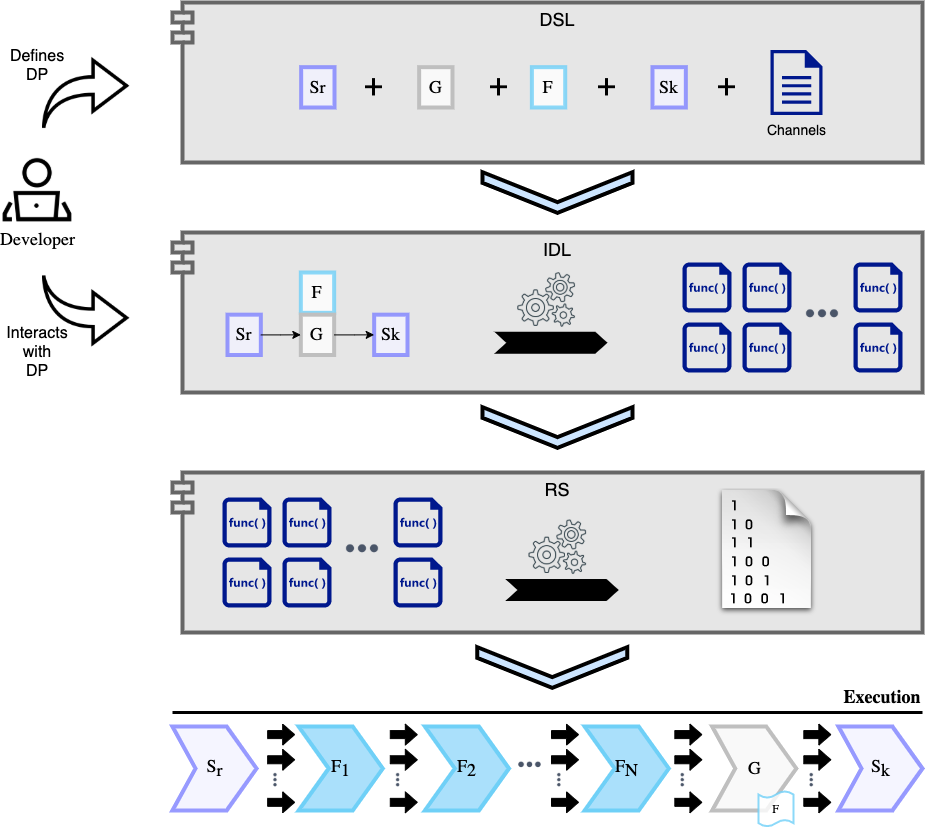
\includegraphics[width=1\textwidth, height=0.6\textheight]{dpf_haskell_v3.png}
    \caption[{[\acrshort{dpfh}] Architectural design of \acrshort{dpfh}}]{This diagram shows the architectural design of \acrshort{dpfh}. \acrshort{dpfh} is a \acrshort{dsl} which is built on three main components: \acrshort{dsl}, \acrshort{idl} and \acrshort{rs}. In the \acrshort{dsl} we can see how the user can compose the main stages of the \acrshort{dp}. \acrshort{idl} is showing how the frameworks is helping the user to transform that definition into real function or computations. Finally \acrshort{rs} execute all that definition plus functions. Execution layer indicates an example of a \acrshort{dp} running after being executed.}
    \label{fig:dpfh:1}
\end{figure}

In \autoref{fig:dpfh:1} we can appreciate the different components mentioned before that are the grey boxes.

\paragraph{DSL} The user interacts with the \acrshort{dsl} component where defines how the \acrshort{dp} flow
should be. Defining the flow consists on to provide a type-level specification about the channels that communicate each stage of the pipeline, as well as the data types those channels carry. 
For example, in the case of \autoref{prole} that we develop the \acrshort{wcc} algorithm, the user knows stages $\iwcc$, $\gwcc$, and $\owcc$ need to be connected with two channels. 
One of those channels is carrying the edges -- \texttt{Edge} data type -- and the other the accumulated connected components -- \texttt{ConnectedComp} data type --. 

\paragraph{IDL} Based on the definition provided in the \acrshort{dsl}, the user interacts with the \acrshort{idl} to build the functions with the algorithms needed for each stage: $\iwcc$, $\gwcc$, $\owcc$, $\fwcc$, and actors. 

\paragraph{RS} \acrshort{rs} is fed with the \acrshort{dp} definition and the functions implementations to finally execute the program. 

\subsection{Implementation}
In this section, we describe the implementation details of each architectural layer: \acrshort{dsl}, \acrshort{idl} and \acrshort{rs}.
As we have explained in \autoref{sec:contrib}, this library was published on Hackage~\cite{dynamic-pipeline}, the source code is open and can be found on this Github Repository~\cite{dynamic-pipeline-git}.

\subsubsection{DSL Grammar}\label{sub:sec:dsl-gram}
In order to provide correctness verification at compilation level, we define a \acrfull{cfg} that generates a \acrshort{dp} \acrshort{dsl} language. 
\acrshort{cfg} enables the user to define a \acrshort{dp} at type-level. 

\begin{definition}[\acrshort{dsl} \acrshort{cfg}]\label{def:cfg:dsl}
Lets $\gdsl = (N, \Sigma, DB, P)$ be a Context-Free Grammar, such that $N$ is the set of non-terminal symbols, $\Sigma$ the set of terminal symbols,
$DP \in N$ is the start symbol and $P$ are the generation rules. \autoref{fig:def:dpfh:dsl} shows the formal definition of the grammar.
\begin{figure}[H]
\begin{equation*}
    \boxed{
      \begin{aligned}
    N &= \{DP,S_r,S_k,G,F_b,CH,CH_s\},\\
    \Sigma &= \{\text{\mintinline{haskell}{Source}},\text{\mintinline{haskell}{Generator}},\text{\mintinline{haskell}{Sink}},\text{\mintinline{haskell}{FeedbackChannel}},\text{\mintinline{haskell}{Type}},\text{\mintinline{haskell}{Eof}},\text{\mintinline{haskell}{:=>}},\text{\mintinline{haskell}{:<+>}}\},
    \end{aligned}
    }
\end{equation*}
\begin{equation*}
  \boxed{
    \begin{aligned}
  P = \{\\
  DP  &\rightarrow S_r\ \text{\mintinline{haskell}{:=>}}\ G\ \text{\mintinline{haskell}{:=>}}\ S_k\ |\ S_r\ \text{\mintinline{haskell}{:=>}}\ G\ \text{\mintinline{haskell}{:=>}}\ F_b\ \text{\mintinline{haskell}{:=>}}\ S_k,\\
  S_r &\rightarrow \text{\mintinline{haskell}{Source}}\ CH_s,\\
  G   &\rightarrow \text{\mintinline{haskell}{Generator}}\ CH_s,\\
  S_k &\rightarrow \text{\mintinline{haskell}{Sink}},\\
  F_b &\rightarrow \text{\mintinline{haskell}{FeedbackChannel}} CH,\\
  CH_s &\rightarrow \text{\mintinline{haskell}{Channel}}\ CH,\\
  CH &\rightarrow \text{\mintinline{haskell}{Type :<+>}}\ CH\ |\ \text{\mintinline{haskell}{Eof}}\}
\end{aligned}
}
\end{equation*}
\caption[{[\acrshort{dpfh}] DSL Grammar definition}]{This is the Context-Free Grammar defined for the DSL. In the first box we can see $N$ which is the set of non-terminals symbols of the Grammar. $\Sigma$ which is the set of the terminal symbols and $P$ the production rules of the grammar.}
\label{fig:def:dpfh:dsl}
\end{figure}
\end{definition}

For encoding $\gdsl$ on the \acrshort{hs}, we use an \emph{Index type}~\cite{type-index} to keep track, at type-level, of the extra information required by the \acrshort{dp} definition such as channels and data types the channels carry. 

\begin{listing}[H]
  \begin{minted}[fontsize=\fontsize{10}{11}\selectfont,numbers=left,breaklines,frame=lines,framerule=2pt,framesep=2mm,baselinestretch=1.2,highlightlines={3,4}]{haskell}

data Source (a :: Type)
data Generator (a :: Type)
data Sink
data Eof
data Channel (a :: Type)
data FeedbackChannel (a :: Type)

  \end{minted}
  \caption[{[\mintinline{shell}{Flow.hs}] $\Sigma$ enconding of $G_{dsl}$}]{This code is showing most of the data types that represent the same terminal symbols $\Sigma \in G_{dsl}$. Those types that are indexed by another kind \mintinline{haskell}{Type}, allows to store information at type-level needed for interpret the DSL}
  \label{src:dpfh:1}
\end{listing}
  
In \autoref{src:dpfh:1}, there is an \emph{Index type} for each element of $\Sigma$ encoded in \acrshort{hs} Types.
The highlighted lines in \autoref{src:dpfh:1} shows the terminal symbols $\Sigma$ that are not indexed, because neither \mintinline{haskell}{Sink} nor \mintinline{haskell}{Eof} are carrying extra type-level information. 
In the case of \mintinline{haskell}{Sink}, since it is the last stage that does not connect further with any other stage, we do not need to indicate any channel information. 
\mintinline{haskell}{Eof} it is just a terminal type to disambiguate the \mintinline{haskell}{Channel (a :: Type)} subtree for the full parser tree. 
\mintinline{haskell}{Channel} can carry any type because it needs to be polymorphic to support a different number of channels and data types.

\begin{listing}[H]
  \begin{minted}[fontsize=\fontsize{10}{11}\selectfont,numbers=left,breaklines,frame=lines,framerule=2pt,framesep=2mm,baselinestretch=1.2,highlightlines={1,5}]{haskell}
    
    data chann1 :<+> chann2 = chann1 :<+> chann2
    deriving (Typeable, Eq, Show, Functor, Traversable, Foldable, Bounded)
    infixr 5 :<+>
    
    data a :=> b = a :=> b
    deriving (Typeable, Eq, Show, Functor, Traversable, Foldable, Bounded)
    infixr 5 :=>
    
  \end{minted}
  \caption[{[\mintinline{shell}{Flow.hs}] $\Sigma$ enconding of $G_{dsl}$ - Especial non-terminals}]{Special terminal symbols $\{\text{\mintinline{haskell}{:<+>}}, \text{\mintinline{haskell}{:=>}}\} \in \Sigma$. This terminal symbols allows to index two types in order to combine several of them and build a chain of stages (\mintinline{haskell}{:=>}) and a set of channels (\mintinline{haskell}{:<+>}).}
  \label{src:dpfh:2}
\end{listing}

There are two important terminal symbols in $\Sigma$: \mintinline{haskell}{:=>} and \mintinline{haskell}{:<+>}.
In \autoref{src:dpfh:2}, the definition shows how \mintinline{haskell}{:=>} and \mintinline{haskell}{:<+>} can combine 2 (two) types. 
The propose of writing \mintinline{haskell}{:=>} and \mintinline{haskell}{:<+>} as types is to have a syntactic sugar type combinator for writing the \acrshort{dsl} according to the \acrshort{cfg}. 
Apart from that, they are different because two distinguishable terminal symbols $\Sigma$ are needed to separate the encoding of the pipeline stage ($\iwcc$, $\gwcc$, $\owcc$)
from the encoding of channel composition in the same stage, as we can appreciate in \dref{def:cfg:dsl}.

Now, we can start defining our pipelines at type-level. For example, if we want to generate a \acrshort{dp} that eliminates duplicated elements in a stream, we know that we only need one channel connecting the stages that carries out the type of the element, in this case, \mintinline{haskell}{Int} (see \autoref{src:dpfh:3}).

\begin{listing}[H]
  \begin{minted}[fontsize=\fontsize{10}{11}\selectfont,numbers=left,breaklines,frame=lines,framerule=2pt,framesep=2mm,baselinestretch=1.2,highlightlines={}]{haskell}

type DPExample = Source (Channel (Int :<+> Eof)) 
              :=> Generator (Channel (Int :<+> Eof)) 
              :=> Sink
   
  \end{minted}
  \caption[{[\mintinline{shell}{Repeated.hs} Example of \acrshort{dp} encoded in $G_{dsl}$}]{This example shows the \acrshort{dsl} encoding in \acrshort{dp} of repeated elements problems}
  \label{src:dpfh:3}
\end{listing}

\subsubsection{DSL Validation}\label{sub:sec:dsl-val}
The language generated by the grammar needs to be validated to avoid errors or provide an incorrect \acrshort{dp} definition.
Fortunately, \acrshort{hs} provides several Type-level techniques~\cite{type-haskell} which allows to verify properties of programs before running them, 
preventing the users to introduce bugs, reducing errors. This verification done by the compiler establish a Curry-Howard Isomorphism~\cite{curryhoward}, i.e. 
\emph{Propositions as Types - Programs as Proof}. It is important to remark here that \acrshort{hs} is not a theorem prover System like Coq~\cite{coq}, but some verifications, as we present in this work, can be done with \acrshort{ghc} to ensure correctness on programs.
Although \acrshort{hs} provides tools to build advanced type-level verifications, all these techniques require the addition of \emph{Haskell Language Extensions}.

Once we have the encoded \acrshort{dp} problem in the \acrshort{dsl} grammar -- see \autoref{sub:sec:dsl-gram} --, we can proceed on validating that encoded grammar. 
The implementation of the validation of the \acrshort{dsl} \acrshort{cfg} at type-level, has been done using \emph{Associated Type Families}~\cite{associated-types}.

\begin{listing}[H]
  \begin{minted}[fontsize=\fontsize{10}{11}\selectfont,numbers=left,breaklines,frame=lines,framerule=2pt,framesep=2mm,baselinestretch=1.2,highlightlines={6,18}]{haskell}

type family And (a :: Bool) (b :: Bool) :: Bool where
    And 'True 'True = 'True
    And a b         = 'False
  

type family IsDP (dpDefinition :: k) :: Bool where
    IsDP (Source (Channel inToGen) :=> Generator (Channel genToOut) :=> Sink)
        = And (IsDP (Source (Channel inToGen))) (IsDP (Generator (Channel genToOut)))
    IsDP ( Source (Channel inToGen) :=> Generator (Channel genToOut) :=> FeedbackChannel toSource :=> Sink)
        = And (IsDP (Source (Channel inToGen))) (IsDP (Generator (Channel genToOut)))
    IsDP (Source (Channel (a :<+> more)))     
        = IsDP (Source (Channel more))
    IsDP (Source (Channel Eof))               = 'True
    IsDP (Generator (Channel (a :<+> more)))  = IsDP (Generator (Channel more))
    IsDP (Generator (Channel a))              = 'True
    IsDP x                                    = 'False
     
type family ValidDP (a :: Bool) :: Constraint where
  ValidDP 'True = ()
  ValidDP 'False = TypeError
                    ( 'Text "Invalid Semantic for Building DP Program"
                      ':$$: 'Text "Language Grammar:"
                      ':$$: 'Text "DP       -> Source CHANS :=> Generator CHANS :=> Sink"
                      ':$$: 'Text "DP       -> Source CHANS :=> Generator CHANS :=> FEEDBACK :=> Sink"
                      ':$$: 'Text "CHANS    -> Channel CH"
                      ':$$: 'Text "FEEDBACK -> FeedbackChannel CH"
                      ':$$: 'Text "CH       -> Type :<+> CH | Eof"
                      ':$$: 'Text "Example: 'Source (Channel (Int :<+> Int)) :=> Generator (Channel (Int :<+> Int)) :=> Sink'"
                    )
  \end{minted}
  \caption[{[\mintinline{shell}{Stage.hs}] Validating encoded in $G_{dsl}$ - FCF}]{Type Families \mintinline{haskell}{And}, \mintinline{haskell}{IsDP} and \mintinline{haskell}{ValidDP} which allows to perform a type-level validation over a \acrshort{dsl} \acrshort{cfg} definition.}
  \label{src:dpfh:4}
\end{listing}

In \autoref{src:dpfh:4}, there are 3(three) Type families that helps to validate the \acrshort{dsl} \acrshort{cfg}. 
\mintinline{haskell}{IsDP} associated type family is checking the production rules $P$ of the grammar defined in \autoref{fig:def:dpfh:dsl}, returning a promoted data type~\cite{promoted-types} (not a boolean value) \mintinline{haskell}{'True} in case
the production rule matches all the generated language, or \mintinline{haskell}{'False} otherwise. 
\mintinline{haskell}{ValidDP} is taking the result of \mintinline{haskell}{IsDP} type application, associating \mintinline{haskell}{'True} promoted boolean type to empty \mintinline{haskell}{()} constraint. An empty constraint is an 
indication of nothing to be restricted, meaning that if \mintinline{haskell}{ValidDP} is used as a constraint, and it is fully applied to \mintinline{haskell}{()}, it will give the compiler the evidence that there is no error at type-level.
\mintinline{haskell}{ValidDP} is also associating \mintinline{haskell}{'False} to a custom \mintinline{haskell}{TypeError} which will appear at compilation time if the \acrshort{dp} \acrshort{dsl} definition fully applies to that.

\begin{listing}[H]
  \begin{minted}[fontsize=\fontsize{10}{11}\selectfont,numbers=left,breaklines,frame=lines,framerule=2pt,framesep=2mm,baselinestretch=1.2,highlightlines={2}]{haskell}

mkDP :: forall dpDefinition filterState filterParam st.
    ( ValidDP (IsDP dpDefinition)
    , DPConstraint dpDefinition filterState st filterParam)
 => Stage (WithSource dpDefinition (DP st)) 
 -> GeneratorStage dpDefinition filterState filterParam st  
 -> Stage (WithSink dpDefinition (DP st))  
 -> DP st ()
mkDP = ...

someFunc = mkDP @DPExample ...

  \end{minted}
  \caption[{[\mintinline{shell}{Stage.hs}] Using validation of \acrshort{dp} encoded in $G_{dsl}$}]{Definition of \mintinline{haskell}{mkDP} function of the Framework which uses type-level validation of the grammar \mintinline{haskell}{ValidDP (IsValid Type)}. Last line of the code is showing that using that function will compile-time check the definition of \mintinline{haskell}{DPExample} type.}
  \label{src:dpfh:5}
\end{listing}

\subsubsection{\acrfull{idl}}
\acrshort{idl} component takes the \acrshort{dp} definition made on with \acrshort{dsl} component to interpret and generate the function definitions
that the user needs to fill in for solving a specific problem. In \autoref{sec:dp}, we have described what the user needs to provide in a \acrshort{dp} algorithm: $\iwcc$, $\gwcc$, $\owcc$, and the $\fwcc$ with the non-empty set of Actors.
The \acrshort{idl} generates the function definitions with an empty implementation to be completed by the user, ensuring that those functions will give "Proof" -- in terms of Curry-Howard Correspondence~\cite{curryhoward} --  of the "Propositions" defined on the \acrshort{dsl}.

Similar techniques that we used on \autoref{sub:sec:dsl-val} are also used here. 
On the first hand, we use \emph{Type-level Defunctionalization}~\cite{defunctionalization, fun-type-function-haskell} to let the compiler generates the signatures of the required functions. 
On the other hand, we use \emph{Term-level Defunctionalization} to interpret those functions.
Moreover, \emph{Indexed Types}~\cite{type-index} and \emph{Heterogeneous List}~\cite{hlist} are used to keep track of the dynamic number and polymorphic types of the functions parameters. 

\begin{listing}[H]
  \begin{minted}[fontsize=\fontsize{10}{11}\selectfont,numbers=left,breaklines,frame=lines,framerule=2pt,framesep=2mm,baselinestretch=1.2,highlightlines={2,6,10}]{haskell}
withSource :: forall (dpDefinition :: Type) st. WithSource dpDefinition (DP st) 
            -> Stage (WithSource dpDefinition (DP st))
withSource = mkStage' @(WithSource dpDefinition (DP st))

withGenerator :: forall (dpDefinition :: Type) (filter :: Type) st. WithGenerator dpDefinition filter (DP st) 
              -> Stage (WithGenerator dpDefinition filter (DP st))
withGenerator = mkStage' @(WithGenerator dpDefinition filter (DP st))

withSink :: forall (dpDefinition :: Type) st. WithSink dpDefinition (DP st) 
           -> Stage (WithSink dpDefinition (DP st))
withSink = mkStage' @(WithSink dpDefinition (DP st))
  \end{minted}
  \caption[{[\mintinline{shell}{Stage.hs}] Using with Interpreters of \acrshort{dp} encoded in $G_{dsl}$}]{This code is showing the different interpreters combinators to help the user to generate the functions of the principal stages of \acrshort{dp}}
  \label{src:dpfh:6}
\end{listing}

In \autoref{src:dpfh:6} we can appreciate the different combinators of the \acrshort{idl} that helps the user of the framework to interpret the \acrshort{dsl} to generate the function definitions.
\mintinline{haskell}{Stage} data type will be cover in \autoref{src:dpfh:8}, but it is a wrapper type of a pipeline stage -- minimal unit of execution --, containing the function to be executed -- here is the use \emph{Term-level Defunctionalization} --.
\mintinline{haskell}{withSource}, \mintinline{haskell}{withGenerator}, and \mintinline{haskell}{withSink} are aliases of the function \mintinline{haskell}{mkStage'} which is the combinator that is applying the \emph{Associated Type} related to that stage. For example \mintinline{haskell}{withSource}, is equivalent to \mintinline{haskell}{mkStage' @(WithSource dpDefinition (DP st))}.
For each \emph{Associated Type Family} defintion, there exist an equivalent term-level definition: \mintinline{haskell}{WithSource} type with \mintinline{haskell}{withSource} term , \mintinline{haskell}{WithGenerator} type with \mintinline{haskell}{withGenerator} term, and \mintinline{haskell}{WithSink} type with \mintinline{haskell}{withSink} term -- notice the capital case letter "W" indicating the type and not the term --.

\begin{listing}[H]
  \begin{minted}[fontsize=\fontsize{10}{11}\selectfont,numbers=left,breaklines,frame=lines,framerule=2pt,framesep=2mm,baselinestretch=1.2,highlightlines={7,11}]{haskell}
type family WithSource (dpDefinition :: Type) (monadicAction :: Type -> Type) :: Type where
  WithSource (Source (Channel inToGen) :=> Generator (Channel genToOut) :=> Sink) monadicAction
      = WithSource (ChanIn inToGen) monadicAction
  WithSource (Source (Channel inToGen) :=> Generator (Channel genToOut) :=> FeedbackChannel toSource :=> Sink) monadicAction 
      = WithSource (ChanOutIn toSource inToGen) monadicAction
  WithSource (ChanIn (dpDefinition :<+> more)) monadicAction         
      = WriteChannel dpDefinition -> WithSource (ChanIn more) monadicAction
  WithSource (ChanIn Eof) monadicAction                              
      = monadicAction ()
  WithSource (ChanOutIn (dpDefinition :<+> more) ins) monadicAction  
      = ReadChannel dpDefinition -> WithSource (ChanOutIn more ins) monadicAction
  WithSource (ChanOutIn Eof ins) monadicAction                       
      = WithSource (ChanIn ins) monadicAction
  WithSource dpDefinition _                                          
      = TypeError
          ( 'Text "Invalid Semantic for Source Stage"
            ':$$: 'Text "in the DP Definition '"
            ':<>: 'ShowType dpDefinition
            ':<>: 'Text "'"
            ':$$: 'Text "Language Grammar:"
            ':$$: 'Text "DP       -> Source CHANS :=> Generator CHANS :=> Sink"
            ':$$: 'Text "DP       -> Source CHANS :=> Generator CHANS :=> FEEDBACK :=> Sink"
            ':$$: 'Text "CHANS    -> Channel CH"
            ':$$: 'Text "FEEDBACK -> FeedbackChannel CH"
            ':$$: 'Text "CH       -> Type :<+> CH | Eof"
            ':$$: 'Text "Example: 'Source (Channel (Int :<+> Int)) :=> Generator (Channel (Int :<+> Int)) :=> Sink'"
          )
  \end{minted}
  \caption[{[\mintinline{shell}{Stage.hs}] WithSource Associate Type Details}]{An example of the Associated Type Family \mintinline{haskell}{WithSource} that allows to implement \emph{Type-level Defunctionalization} technique that will be the Type-level verification of the term \mintinline{haskell}{withSource}}
  \label{src:dpfh:7}
\end{listing}

In \autoref{src:dpfh:7}, in the highlighted lines, it can be seen how \emph{Type-level Defunctionalization} is being expanded in a signature function definition with the form \mintinline{haskell}{WriteChannel a -> ReadChannel b -> ... -> monadicAction ()} depending on \acrshort{dp} language definition. 

\begin{listing}[H]
  \begin{minted}[fontsize=\fontsize{10}{11}\selectfont,numbers=left,breaklines,frame=lines,framerule=2pt,framesep=2mm,baselinestretch=1.2,highlightlines={12,16}]{haskell}

data Stage a where
  Stage :: Proxy a -> a -> Stage a

mkStage' :: forall a. a -> Stage a
mkStage' = Stage (Proxy @a)
    
  \end{minted}
  \caption[{[\mintinline{shell}{Stage.hs}] Stage Data Type}]{\mintinline{haskell}{Stage} data type for implementing \emph{Term-level Defunctionalization} providing evidence to the Type-Level Associated types}
  \label{src:dpfh:8}
\end{listing}

In \autoref{src:dpfh:8}, \mintinline{haskell}{Stage} data type uses a \mintinline{haskell}{Proxy} phantom type. 
This phantom type allow \mintinline{haskell}{Stage} to index the type definition generated by \mintinline{haskell}{a}.
For example, in \autoref{src:dpfh:6}, when \mintinline{haskell}{withSource} interpreter is applied to \mintinline{haskell}{WithSource dpDefinition},  
the compiler is provided with \mintinline{haskell}{dpDefinition} \acrshort{dsl} type, it expands the function signature belonging to that \acrshort{dp} definition inside the \mintinline{haskell}{Stage}.

\paragraph{Generator and Filter}
According to \acrshort{dp} definition in \autoref{sec:dp}, $\gwcc$ has a $\fwcc$ template in order to know how to dynamically interpose a new $\fwcc$ during the runtime execution of the program.
Let's first study $\fwcc$ Data Type in the context of the framework.

\begin{listing}[H]
  \begin{minted}[fontsize=\fontsize{10}{11}\selectfont,numbers=left,breaklines,frame=lines,framerule=2pt,framesep=2mm,baselinestretch=1.2,highlightlines={2,5}]{haskell}

newtype Actor dpDefinition filterState filterParam monadicAction =
    Actor {  unActor :: MonadState filterState monadicAction => Stage (WithFilter dpDefinition filterParam monadicAction) }

newtype Filter dpDefinition filterState filterParam st =
    Filter { unFilter :: NonEmpty (Actor dpDefinition filterState filterParam (StateT filterState (DP st))) }
    deriving Generic
    
  \end{minted}
  \caption[{[\mintinline{shell}{Stage.hs}] Filter / Actor Data Type}]{This code shows the definition of the \mintinline{haskell}{Filter} data type which contains a non-empty set of \mintinline{haskell}{Actor}. The \mintinline{haskell}{Actor} data type is an \mintinline{haskell}{Stage} in the Context of the \mintinline{haskell}{MonadState} to allow keeping a local memory in the execution context of the filter.}
  \label{src:dpfh:9}
\end{listing}

In \autoref{src:dpfh:9} the definition of the \mintinline{haskell}{Filter} data type contains a non-empty set of \mintinline{haskell}{Actor}.
An \mintinline{haskell}{Actor} is a \mintinline{haskell}{Stage}, because an actor is the minimal unit of execution of a filter. 
A \mintinline{haskell}{Filter} has a \mintinline{haskell}{NonEmpty Actor} -- Non-empty List -- because a filter is built by a sequence of actors calls. 
Moreover, \mintinline{haskell}{Actor} Stage is defunctionalized with \mintinline{haskell}{WithFilter} \emph{Associated Type Family}. 
\mintinline{haskell}{Filter} runs in an explicit \mintinline{haskell}{StateT} monadic context. This is because the $\fwcc$ instance should have an state, according to \acrshort{dp} definition in \autoref{sec:dp}.
For example, in the case of $\dpwcc$, as we have seen in \autoref{prole}, $\fwcc$ keeps an updated list of connected components that updates as long as it receives more edges that are connected with the current list of vertices.
\mintinline{haskell}{Actor} data type -- see \autoref{src:dpfh:9} --, is constrained by \mintinline{haskell}{MonadState} which is in the same execution context of the whole \mintinline{haskell}{NonEmpty Actor} list of the \mintinline{haskell}{Filter}. 
This means the \mintinline{haskell}{StateT} is executed for each \mintinline{haskell}{Actor} of that filter, sharing the same state between them. 

\begin{listing}[H]
  \begin{minted}[fontsize=\fontsize{10}{11}\selectfont,numbers=left,breaklines,frame=lines,framerule=2pt,framesep=2mm,baselinestretch=1.2,highlightlines={}]{haskell}

mkFilter :: forall dpDefinition filterState filterParam st. WithFilter dpDefinition filterParam (StateT filterState (DP st)) 
         -> Filter dpDefinition filterState filterParam st
mkFilter = Filter . single

single :: forall dpDefinition filterState filterParam st. WithFilter dpDefinition filterParam (StateT filterState (DP st)) 
       -> NonEmpty (Actor dpDefinition filterState filterParam (StateT filterState (DP st)))
single = one . actor

actor :: forall dpDefinition filterState filterParam st. WithFilter dpDefinition filterParam (StateT filterState (DP st)) 
      -> Actor dpDefinition filterState filterParam (StateT filterState (DP st))
actor = Actor . mkStage' @(WithFilter dpDefinition filterParam (StateT filterState (DP st)))

(|>>>) :: forall dpDefinition filterState filterParam st. Actor dpDefinition filterState filterParam (StateT filterState (DP st)) 
       -> Filter dpDefinition filterState filterParam st 
       -> Filter dpDefinition filterState filterParam st
(|>>>) a f = f & _Wrapped' %~ (a <|)
infixr 5 |>>>

(|>>) :: forall dpDefinition filterState filterParam st. Actor dpDefinition filterState filterParam (StateT filterState (DP st)) 
      -> Actor dpDefinition filterState filterParam (StateT filterState (DP st)) 
      -> Filter dpDefinition filterState filterParam st
(|>>) a1 a2 = Filter (a1 <|one a2)
infixr 5 |>>
  \end{minted}
  \caption[{[\mintinline{shell}{Stage.hs}] Filter / Actor smart constructors and combinators}]{Combinators and small constructor to enable building actors and filter.}
  \label{src:dpfh:10}
\end{listing}

Finally, in \autoref{src:dpfh:10}, some combinators and smart constructors are provided in the framework to enable the construction of \mintinline{haskell}{Filter} and \mintinline{haskell}{Actor}.
\mintinline{haskell}{mkFilter} is a smart constructor for \mintinline{haskell}{Filter} Data Constructor. \mintinline{haskell}{single} wraps one actor inside a \mintinline{haskell}{Filter}.
\mintinline{haskell}{actor} is a smart constructor for \mintinline{haskell}{Actor} Data Constructor. \mintinline{haskell}{(|>>>)} is an appending combinator of an \mintinline{haskell}{Actor} to a \mintinline{haskell}{Filter}. 
\mintinline{haskell}{(|>>>)} also ensures actor execution order, i.e. the latest actor added is the latest to be executed.


\begin{listing}[H]
  \begin{minted}[fontsize=\fontsize{10}{11}\selectfont,numbers=left,breaklines,frame=lines,framerule=2pt,framesep=2mm,baselinestretch=1.2,highlightlines={}]{haskell}
    data GeneratorStage dpDefinition filterState filterParam st = GeneratorStage
    { _gsGenerator      :: Stage (WithGenerator dpDefinition (Filter dpDefinition filterState filterParam st) (DP st))
    , _gsFilterTemplate :: Filter dpDefinition filterState filterParam st
    }  
  \end{minted}
  \caption[{[\mintinline{shell}{Stage.hs}] Generator}]{\mintinline{haskell}{Generator} Data type which contains the \mintinline{haskell}{Stage} code of the generator itself, and the \mintinline{haskell}{Filter} template that it can be spawned by the \mintinline{haskell}{Generator}.}
  \label{src:dpfh:11}
\end{listing}

In \autoref{src:dpfh:11}, $\gwcc$ contains a $\fwcc$ template and its own stage behavior.
\mintinline{haskell}{Generator} data type has a field with the \mintinline{haskell}{Filter} template that could be spawned by the algorithm defined by the user according to the data received from its input channels.
\mintinline{haskell}{Generator} has also another field with the behavior of the $\gwcc$ -- a \mintinline{haskell}{Stage} --. 

\subsubsection{\acrfull{rs}}
The \acrshort{rs} can be divided into two parts: the mechanism to generate stages dynamically in runtime, and the execution entry point of the \acrshort{dp}.
Regarding execution entry point, all the stages that we have seen in previous sections are the pieces needed to build an executable \mintinline{haskell}{DP st a} monad.
This executable monad has an existential type similar to \mintinline{haskell}{ST} monad to not escape out from the context on different stages.
Once the dynamic pipeline starts to execute, the core of the framework dynamically generates stages between $\gwcc$ and previous stages, according to the user definition, i.e. an \emph{anamorphism}~\cite{lenses} that creates $\fwcc$ instances until some condition is met.

\begin{listing}[H]
  \begin{minted}[fontsize=\fontsize{10}{11}\selectfont,numbers=left,breaklines,frame=lines,framerule=2pt,framesep=2mm,baselinestretch=1.2,highlightlines={2,12,14,15,16,17,18}]{haskell}
unfoldF :: forall dpDefinition readElem st filterState filterParam l. SpawnFilterConstraint dpDefinition readElem st filterState filterParam l
        => UnFoldFilter dpDefinition readElem st filterState filterParam l 
        -> DP st (HList l) 
unfoldF = loopSpawn

where
  loopSpawn uf@UnFoldFilter{..} =
    maybe (pure _ufRsChannels) (loopSpawn <=< doOnElem uf) =<< DP (pull _ufReadChannel)

  doOnElem uf@UnFoldFilter{..} elem' = do
    _ufOnElem elem'
    if _ufSpawnIf elem'
     then do
       (reads', writes' :: HList l3) <- getFilterChannels <$> DP (makeChansF @(ChansFilter dpDefinition))
       let hlist = elem' .*. _ufReadChannel .*. (_ufRsChannels `hAppendList` writes')
       void $ runFilter _ufFilter (_ufInitState elem') hlist (_ufReadChannel .*. (_ufRsChannels `hAppendList` writes'))
       return $ uf { _ufReadChannel = hHead reads', _ufRsChannels = hTail reads' }
     else return uf

  \end{minted}
  \caption[{[\mintinline{shell}{Stage.hs}] unfoldF}]{\mintinline{haskell}{unfolF} is the \emph{anamorphism} combinator to spawn new \mintinline{haskell}{Filter} types between the \mintinline{haskell}{Generator} and previous stages.}
  \label{src:dpfh:12}
\end{listing}

In \autoref{src:dpfh:12}, it is presented how is the \emph{anamorphism} mechanims that generates dynamic stages between $\gwcc$ and the previous stages.
That \emph{anamorphism} is implemented with the function \mintinline{haskell}{unfoldF}. That function receives an \mintinline{haskell}{UnFoldFilter} Data type, which contains the recipe for controlling that unfold recursive call. 
In line $12$, \mintinline{haskell}{_ufSpawnIf} field of \mintinline{haskell}{UnFoldFilter}, indicates when to stop the recursion. 
Inside the conditional, in line $14$, new channels are created for the new filter to be spawned. Those new channels connect the new filter with the previous stages and with \mintinline{haskell}{Generator}. 
After that, in line $16$ \mintinline{haskell}{runFilter} starts the monadic computation, spawning the filter stage with its actors.
Finally, the new list of channels are returned for the next recursive step to allow further channel connections.

\begin{listing}[H]
  \begin{minted}[fontsize=\fontsize{10}{11}\selectfont,numbers=left,breaklines,frame=lines,framerule=2pt,framesep=2mm,baselinestretch=1.2,highlightlines={}]{haskell}
mkUnfoldFilter :: (readElem -> Bool) 
    -> (readElem -> DP st ()) 
    -> Filter dpDefinition filterState filterParam st 
    -> (readElem -> filterState)
    -> ReadChannel readElem
    -> HList l 
    -> UnFoldFilter dpDefinition readElem st filterState filterParam l


mkUnfoldFilterForAll' :: (readElem -> DP st ())
                      -> Filter dpDefinition filterState filterParam st
                      -> (readElem -> filterState)
                      -> ReadChannel readElem
                      -> HList l
                      -> UnFoldFilter dpDefinition readElem st filterState filterParam l

mkUnfoldFilterForAll :: Filter dpDefinition filterState filterParam st
                      -> (readElem -> filterState)
                      -> ReadChannel readElem
                      -> HList l
                      -> UnFoldFilter dpDefinition readElem st filterState filterParam l
   \end{minted}
  \caption[{[\mintinline{shell}{Stage.hs}] UnfoldFilter combinators}]{Combinators for building \mintinline{haskell}{UnfoldFilter} types indicating the type of the \mintinline{haskell}{unfold} that the user want to achieve.}
  \label{src:dpfh:13}
\end{listing}

Several smart constructors are also provided for building \mintinline{haskell}{UnfoldFilter} Data Type.
In \autoref{src:dpfh:13} the first combinator is the default smart constructor.  \begin{inparaenum}[i\upshape)]
  \item First field \mintinline{haskell}{(readElem -> Bool)} indicate if the a new filter should be spawn or not.
  \item Second field \mintinline{haskell}{(readElem -> DP st ())} is a monadic optional computation to do when received a new element, for example logging.
  \item Third field \mintinline{haskell}{Filter} data type to be spawned.
  \item Fourth field \mintinline{haskell}{(readElem -> filterState)} is initialization of the \mintinline{haskell}{Filter} State.
  \item Fifth field \mintinline{haskell}{(ReadChannel readElem)} that feeds the filter instance.
  \item Last field is the \emph{Heterogeneous List} with the rest of the channels to connect with other stages.
\end{inparaenum}.
The combinator \mintinline{haskell}{mkUnfoldFilterForAll} is an smart constructor of \mintinline{haskell}{UnfoldFilter} that allows to spawn a new filter for each element received in the $\gwcc$.

\subsection{Libraries and Tools}
\subsection{Parallelization} 
One of the most important components of the implementation is the selection of concurrency libraries to support an intensive parallelization workload. Parallelization techniques and tools have been intensively studied and implemented in \acrshort{hs} \cite{monadpar}. 
Indeed, it is well known that green threads and sparks allow spawning thousands to millions of parallel computations. 
These parallel computations do not penalize performance when compare with \acrfull{os} level threading \cite{parallelbook}. 
A straightforward assumption to achieve here, is to use \texttt{monad-par} library \cite{monadparlib, monadpar}. 
Nevertheless, in this work, we have discarded the use of sparks \cite{sparks} because we can achieve the level of required parallelism spawning green threads only.
The next obvious choice is to use \mintinline{haskell}{forkIO :: IO () -> IO ThreadId} from \texttt{base} library \cite{forkio}. 
However, that would imply handling all the threads lifecycles and errors programmatically without any abstraction to facilitate that complex task. 
Therefore, we choose \texttt{async} library \cite{async} which enables to spawn asynchronous computations \cite{parallelbook} on \acrshort{hs} using green threads, and at the same time, it provides useful combinators to managing thread terminations and errors.

\subsubsection{Channels\label{section:channels}} 
We have several techniques to our disposal to communicate between threads or sparks in \acrshort{hs} like \mintinline{haskell}{MVar} or concurrent safe mechanisms like \acrfull{stm} \cite{stm}. 
At the same time, in \acrshort{hs} library ecosystem, we dispose of \texttt{Channels} abstractions based on both mentioned communication techniques. 
In that sense, for conducting the communication between dynamic stages and data flowing in a \acrshort{dp}, we have selected \texttt{unagi-chan} library \cite{unagi} which provides the following advantages to our solution: Firstly, \mintinline{haskell}{MVar} channel without using \acrshort{stm} reducing overhead. 
\acrshort{stm} is not required in a \acrshort{dp} because one specific stage which is running in a separated thread, can only access to its \texttt{I/O} channels for reading/writing accordingly, and those operations are not concurrently shared by other threads (stages) for the same channels. 
Second, non-blocking channels. \texttt{unagi-chan} library contains blocking and non-blocking channels for reading. This aspect is key to gain speed up on the implementation. Third, the library is optimized for $x86$ architectures with use of low-level \texttt{fetch-and-add} instructions. Finally, \texttt{unagi-chan} is $100x$ faster~\cite{unagi-bench} on Benchmarking compare with \acrshort{stm} and default base \mintinline{haskell}{Chan} implementations.


\iffalse
\subsection{\texorpdfstring{$\dpwcc$}{Lg} Algorithm}\label{sub:sec:wcc:algo}
Let us consider the problem of computing/enumerating the (weak) connected components of a graph $G$ using \acrshort{dp}. 
A connected component of a graph is a subgraph in which any two vertices are connected by paths.  
Thus, finding connected components of an undirected graph implies obtaining the minimal partition of the set of nodes induced by the relationship \textit{connected}, i.e., there is a path between each pair of nodes. 
An example of that graph can be seen in \autoref{fig:example_dp_graph}.
The input of the Dynamic Pipeline for computing the WCC of a graph, $\dpwcc$, is a sequence of edges ending with $\eof$\footnote{Note that there are neither isolated vertices nor loops in the source graph $G$.}. 
The connected components are output as soon as they are computed, i.e., they are produced incrementally. 
Roughly speaking the idea of the algorithm is that the weakly connected components are built in two phases. 
In the first phase filter instance stages receive the edges of the input graph and create sets of connected vertices. 
During the second phase, these filter instances construct maximal subsets of connected vertices, i.e. the vertices corresponding to (weakly) connected components.
%
$\dpwcc$ is defined in terms of the behavior of its four kinds stages: \textit{Source} ($\iwc$),  \textit{Generator} ($\gwc$),  \textit{Sink} ($\owc$), and \textit{Filter}($\fwc$) stages. Additionally,  the channels connecting these stages must be defined. 
In $\dpwcc$, stages are connected linearly and unidirectionally through the channels $\ice$ and  $\csofv$. Channel $\ice$ carries edges while channel  $\csofv$ conveys sets of connected vertices. Both channels end by the $\eof$ mark. 
The behavior of $\fwc$ is given by a sequence of two actors (scripts). Each actor corresponds to a phase of the algorithm. In what follows, we denote these actors by $\Act$ and $\Actt$, respectively. 
The script $\Act$ keeps a set of connected vertices ($CV$) in the state of the $\fwc$ instance. When an edge $e$ arrives, if an endpoint of $e$ is present in the state, then the other endpoint of $e$ is added to $CV$. 
Edges without incident endpoints are passed to the next stage. When $\eof$ arrives at channel $\ice$, it is passed to the next stage, and the script $\Actt$ starts its execution. 
If script $\Actt$ receives a set of connected vertices $CV$ in $\csofv$, it determines if the intersection between $CV$ and the nodes in its state is not empty. If so, it adds the nodes in $CV$  to its state. 
Otherwise, the $CV$ is passed to the next stage. Whenever $\eof$ is received, $\Actt$ passes--through $\csofv$-- the set of vertices in its state and the $\eof$ mark to the next stage; then, it dies.
The behavior of $\iwc$ corresponds to the identity transformation over the data stream of edges.  As edges arrive, they are passed through  $\ice$ to the next stage. When receiving $\eof$ on $\ice$, this mark is put on both channels. 
Then, $\iwc$ dies. 

%\begin{wrapfigure}{r}{0.4\textwidth}
\begin{figure}
 \begin{center}
\inputtikz{graph_example_wcc}
\end{center}
\caption[{[PoC] Graph WCC Example}]{Example of a graph with two weakly connected components: $\{1,2\}$ and $\{3,4,5,6\}$}
\label{fig:example_dp_graph}
\end{figure}
%\end{wrapfigure}

Let us describe this behavior with the example of the graph shown in \autoref{fig:example_dp_graph}.

\begin{figure}[h!]
  \centering
\inputtikz{dp_example_0}
\caption[{[PoC] $\dpwcc$ Initial Setup}]{$\dpwcc$ Initial setup. Stages Source, Generator, and Sink are represented by the squares labeled by $\mathsf{Sr_{WCC}}$, $\mathsf{G_{WCC}}$ and $\mathsf{Sk_{WCC}}$, respectively.  The square $\fwc$ corresponding to the Filter stage template is the parameter of $\gwc$. Arrows $\rightrightarrows$ between represents the connection of stages through two channels, $\ice$, and $\csofv$. The arrow  $\rightarrow$ represents the channel $\csofv$ connecting the stages $\mathsf{G_{WCC}}$ and $\mathsf{Sk_{WCC}}$. The arrow $\Longrightarrow$ stands for I/O data flow. Finally, the input stream comes between the dotted lines on the left and the WCC computed incrementally will be placed between the solid lines on the right.}
\label{fig:dp_example_0}
\end{figure}

\autoref{fig:dp_example_0} depicts the initial configuration of $\dpwcc$. 
The interaction of $\dpwcc$ with the "external" world is done through the stages $\iwc$ and $\owc$. 
Indeed, once activated the initial $\dpwcc$, the input stream -- consisting of a sequence containing all the edges in the graph in \autoref{fig:example_dp_graph} -- feeds $\iwc$ while  $\owc$ emits incrementally the resulting weakly connected components.  
In what follows \autoref{fig:dp_example_1_2}, \autoref{fig:dp_example_3_4}, \autoref{fig:dp_example_5_6}, \autoref{fig:dp_example_7_8} and \autoref{fig:dp_example_9_10} depict the evolution of the $\dpwcc$.
 
\begin{figure}[h!]
\centering
\begin{subfigure}[b]{\textwidth}
 \centering
  \inputtikz{dp_example_1}
  \caption{The edge $(1,2)$ is arriving to $\gwc$.}
  \label{fig:dp_example_1_2a}
\end{subfigure}
\vspace{.3cm}

\begin{subfigure}[b]{\textwidth}
 \centering
  \inputtikz{dp_example_2}
  \caption{When the edge $(1,2)$ arrives to $\gwc$, it  spawns a new instance of $\fwc$ before $\gwc$. Filter instance $F_{\{1,2\}}$ is connected to  $\gwc$ through channels $\ice$ and  $\csofv$. The state of the new filter instance $F_{\{1,2\}}$ is initialized with the set of vertices $\{1,2\}$. The edge $(3,6)$ arrives to the new filter instance $F_{\{1,2\}}$.}
  \label{fig:dp_example_1_2b}
\end{subfigure}
\caption[{[PoC] $\dpwcc$ Evolving first state}]{Evolution of the $\dpwcc$: First state}
\label{fig:dp_example_1_2}
\end{figure}
\vspace{.5cm}

\begin{figure}[h!]
\centering
\begin{subfigure}[b]{\textwidth}
 \centering
  \inputtikz{dp_example_3}
  \caption{None of the vertices in the edge $(3,6)$ is in the set of vertices $\{1,2\}$ in the state of $F_{\{1,2\}}$, hence it is passed through $\ice$ to $\gwc$.}
  \label{fig:dp_example_3_4a}
\end{subfigure}
\vspace{.3cm}

\begin{subfigure}[b]{\textwidth}
 \centering
  \inputtikz{dp_example_4}
  \caption{When the edge $(3,6)$ arrives to $\gwc$, it spawns the filter instance $F_{\{3,6\}}$  between $F_{\{1,2\}}$ and $\gwc$. Filter instance $F_{\{1,2\}}$ is connected to the new filter instance $F_{\{3,6\}}$ and this one is connected to  $\gwc$ through channels $\ice$ and  $\csofv$. The state of the new filter instance $F_{\{3,6\}}$ is initialized with the set of vertices $\{3,6\}$. The edge $(3,4)$ arrives to $F_{\{1,2\}}$  and $\mathsf{Sr_{WCC}}$ is fed with the mark $\eof$. Edges $(3,4)$ and $(4,5)$ remain passing through $\ice$.}
  \label{fig:dp_example_3_4b}
\end{subfigure}
\caption[{[PoC] $\dpwcc$ Evolving second state}]{Evolution of the $\dpwcc$: Second state}
\label{fig:dp_example_3_4}
\end{figure}
\vspace{.5cm}

\begin{figure}[h!]
\centering
\begin{subfigure}[b]{\textwidth}
 \centering
  \inputtikz{dp_example_5}
  \caption{$\mathsf{Sr_{WCC}}$  fed both, $\ice$ and $\csofv$, channels with the mark $\eof$ received from the input stream in previous state and then, it died. The edge $(4,5)$ is arriving to $\gwc$ and the edge $(3,4)$ is arriving to $F_{\{3,6\}}$. }
  \label{fig:dp_example_5_6a}
\end{subfigure}
\vspace{.3cm}

\begin{subfigure}[b]{\textwidth}
 \centering
  \inputtikz{dp_example_6}
  \caption{When the edge $(4,5)$ arrives to $\gwc$, it spawns the filter instance $F_{\{4,5\}}$  between $F_{\{3,6\}}$ and $\gwc$. Filter instance $F_{\{3,6\}}$ is connected to the new filter instance $F_{\{4,5\}}$ and this one is connected to  $\gwc$ through channels $\ice$ and  $\csofv$.  Since the edge $(3,4)$ arrived to $F_{\{3,6\}}$ at the same time and  vertex $3$ belongs to the set of connected vertices of the filter $F_{\{3,6\}}$,  the vertex $4$ is added to the state of $F_{\{3,6\}}$. Now, the state of $F_{\{3,6\}}$ is the connected set of vertices $\{3,4,6\}$. When the mark $\eof$ arrives to the first filter instance, $F_{\{1,2\}}$, through  $\csofv$, this stage passes  its partial set of connected vertices,  $\{1,2\}$, through $\csofv$ and dies.  This action will activate $\Actt$ in next  filter instances to start building  maximal connected components. In this example, the state in  $F_{\{3,6\}}$, $\{3,4,6\}$, and the arriving set $\{1,2\}$ do not intersect and, hence, both sets of vertices, $\{1,2\}$ and $\{3,4,6\}$ will be passed  to the next filter instance through $\csofv$.}
  \label{fig:dp_example_5_6b}
\end{subfigure}
\caption[{[PoC] $\dpwcc$ Evolving third state}]{Evolution of the $\dpwcc$: Third state}
\label{fig:dp_example_5_6}
\end{figure}
\vspace{.5cm}

\begin{figure}[h!]
\centering
\begin{subfigure}[b]{\textwidth}
 \centering
  \inputtikz{dp_example_7}
  \caption{The set of connected vertices  $\{3,4,6\}$ is arriving to $F_{\{4,5\}}$. The mark $\eof$ continues passing to next stages through the channel $\ice$.}
  \label{fig:dp_example_7_8a}
\end{subfigure}
\vspace{.3cm}

\begin{subfigure}[b]{\textwidth}
 \centering
  \inputtikz{dp_example_8}
  \caption{Since the intersection of the set of connected vertices $\{3,4,6\}$ arrived to  $F_{\{4,5\}}$ and its state is not empty, this state is enlarged to be $\{3,4,5,6\}$. The set of connected vertices $\{1,2\}$ is arriving to  $F_{\{4,5\}}$}
  \label{fig:dp_example_7_8b}
\end{subfigure}
\caption[{[PoC] $\dpwcc$ Evolving fourth state}]{Evolution of the $\dpwcc$:  Fourth state}
\label{fig:dp_example_7_8}
\end{figure}
\vspace{.5cm}

\begin{figure}[h!]
\centering
\begin{subfigure}[b]{\textwidth}
 \centering
  \inputtikz{dp_example_9}
  \caption{$F_{\{4,5\}}$ has passed the set of connected vertices  $\{1,2\}$ and it is arriving to $\mathsf{Sk_{WCC}}$. The mark $\eof$ is arriving to  $F_{\{4,5\}}$ through $\csofv$.}
  \label{fig:dp_example_9_10a}
\end{subfigure}
\vspace{.3cm}

\begin{subfigure}[b]{\textwidth}
 \centering
  \inputtikz{dp_example_10}
  \caption{Since the mark $\eof$ arrived to $F_{\{4,5\}}$ through $\csofv$, it passes its state, the set $\{3,4,5,6\}$ through $\csofv$ to next stages and died. The set of connected vertices  $\{1,2\}$ arrived to $\mathsf{Sk_{WCC}}$ and this implies  that $\{1,2\}$ is a maximal set of connected vertices, i.e. a connected component of the input graph. Hence,  $\mathsf{Sk_{WCC}}$ output this first weakly connected component.}
 \label{fig:dp_example_9_10b}
\end{subfigure}
\vspace{.5cm}

\begin{subfigure}[b]{\textwidth}
 \centering
  \inputtikz{dp_example_11}
  \caption{Finally, the set of connected vertices  $\{3,4,5,6\}$ arrived to $\mathsf{Sk_{WCC}}$ and was output as a new weakly connected component. Besides, the mark $\eof$ also arrived to $\mathsf{Sk_{WCC}}$ through $\csofv$ and thus, it dies.}
  \label{fig:dp_example_9_10c}
\end{subfigure}
\vspace{.3cm}

\begin{subfigure}[b]{\textwidth}
 \centering
  \inputtikz{dp_example_12}
  \caption{The weakly connected component of in the graph \autoref{fig:example_dp_graph} such as they have been emitted by $\dpwcc$.}
  \label{fig:dp_example_9_10d}
\end{subfigure}
\caption[{[PoC] $\dpwcc$ Evolving last state}]{Last states in the evolution of the $\dpwcc$}
\label{fig:dp_example_9_10}
\end{figure}

It is importat to highlight that during the states shown in \autoref{fig:dp_example_1_2a},  \autoref{fig:dp_example_1_2b},  \autoref{fig:dp_example_3_4a},  \autoref{fig:dp_example_3_4b} and  \autoref{fig:dp_example_5_6a} the only actor executed in any filter instance is $\Act$ (constructing sets of connected vertices). Afterwards, although $\Act$ can continue being executed in some filter instances, there are some instances that start executing $\Actt$ (constructing sets of maximal connected vertices). This is shown from \autoref{fig:dp_example_5_6a}  to \autoref{fig:dp_example_9_10a}.
\fi
%
\section{Enumerating Weakly Connected Component on the DPF}\label{sec:wcc-dpf}
This section presents the most relevant details of the implementation of the $\dpwcc$ using DPF-Haskell. 
The $\dpwcc$ implementation has been made as a proof of concept to understand and explore the limitations and challenges that we could find in the development of a future \acrshort{dpf} in \acrshort{hs}. 
In Section \ref{dp-hs}, we emphasize that the focus of \acrshort{dpf} in \acrshort{hs} is on the \acrshort{idl} component. 
Hence, the development of the $\dpwcc$ is as general as possible, using most of the constructs and abstractions required by the \acrshort{idl}. 
Next, we present the minimal code needed for encoding any \acrshort{dp} using \acrshort{dpfh}. \footnote{All the code that we expose here can be accessed publicly in \url{https://github.com/jproyo/dynamic-pipeline/tree/main/examples/Graph}}

\begin{listing}[H]
  \begin{minted}[fontsize=\fontsize{10}{11}\selectfont,numbers=left,breaklines,frame=lines,framerule=2pt,framesep=2mm,baselinestretch=1.2,highlightlines={1-3,6}]{haskell}
    
    type DPConnComp = Source (Channel (Edge :<+> ConnectedComponents :<+> Eof))
                :=> Generator (Channel (Edge :<+> ConnectedComponents :<+> Eof))
                :=> Sink

    program :: FilePath -> IO ()
    program file = runDP $ mkDP @DPConnComp (source' file) generator' sink'
        
  \end{minted}
  \caption[{[\mintinline{shell}{ConnectedComp.hs}] Main entry point of the program}]{In this code we can appreciate the main construct of our $\dpwcc$ which is a combination of $\iwc$, $\gwc$ and $\owc$}
  \label{src:dpwcc:1}
\end{listing}

In \autoref{src:dpwcc:1}, there are two important declarations. First, the \textit{Type Level} declaration of the $\dpwcc$ to indicate \acrshort{dpfh} how our stages are going be connected, and
using that \textit{Type Level} construct, we use the \acrshort{idl} to allow the framework interpret the type representation of our \acrshort{dp} and ensuring at compilation time that we provide the correct stages,  \textit{Source} ($\iwc$), \textit{Generator} ($\gwc$) and \textit{Sink} ($\owc$), that matches those declaration. As we can see in \autoref{src:dpwcc:1}, highlighted lines $1$-$3$ matches one to one the definition in \autoref{fig:dp_example_0}, although in the case of the framework it is not required to provide \textit{Filter} ($\fwc$) definition because \acrshort{dpfh} will deducted from \mintinline[breaklines]{haskell}{Generator}.
According to this declaration what we need to provide is the correct implementation of \mintinline{haskell}{source'}, \mintinline{haskell}{generator'} and \mintinline{haskell}{sink'}
which \textit{Type checked} the \acrshort{dp} type definition\footnote{The names of the functions are completely choosen by the user of the framework and it should not be confused with the internal framework combinators.}.

\begin{listing}[H]
  \begin{minted}[fontsize=\fontsize{10}{11}\selectfont,numbers=left,breaklines,frame=lines,framerule=2pt,framesep=2mm,baselinestretch=1.2,highlightlines={4-5,8}]{haskell}
    
    source' :: FilePath
            -> Stage
              (WriteChannel Edge -> WriteChannel ConnectedComponents -> DP st ())
    source' filePath = withSource @DPConnComp
      $ \edgeOut _ -> unfoldFile filePath edgeOut (toEdge . decodeUtf8)

    sink' :: Stage (ReadChannel Edge -> ReadChannel ConnectedComponents -> DP st ())
    sink' = withSink @DPConnComp $ \_ cc -> withDP $ foldM_ cc print

    generator' :: GeneratorStage DPConnComp ConnectedComponents Edge st
    generator' =
      let gen = withGenerator @DPConnComp genAction
      in  mkGenerator gen filterTemplate
        
  \end{minted}
  \caption[{[\mintinline{shell}{ConnectedComp.hs}] $\iwc$, $\gwc$ $\owc$ Code}]{In this code we can appreciate the $\iwc$, $\gwc$ and $\owc$ functions that matches the type level definition of the $\DP$. $\iwc$ and $\owc$ are completely trivial but $\gwc$ will be analyzed later due to its internal complexity.}
  \label{src:dpwcc:2}
\end{listing}

As we appreciate in \autoref{src:dpwcc:2}, $\iwc$ and $\owc$ are trivial. In the case of \mintinline{haskell}{source'} the only work it needs to do is to read the input data edge by edge and downstream to the next stages. 
That process is achieved with a \acrshort{dpfh} combinator called \mintinline{haskell}{unfoldFile} which is a \emph{catamorphism} of the input data to the stream.
\mintinline{haskell}{sink'} delivers to the output of the program the upstream connected components received from previous stages. $\owc$ implementation is done using an \emph{anamorphism} combinator provided by the framework as well, which is \mintinline{haskell}{foldM_}.
The $\gwc$ Stage is a little more complex because it contains the core of the algorithm explained in \autoref{prole}. According to what we described in \autoref{sec:dp}, \textit{Generator} stage spawns a \textit{Filter} on each received edge in our case of $\dpwcc$.
Therefore, it needs to contain that recipe on how to generate a new \textit{Filter} instance -- in our case of \acrshort{hs} it is a defunctionalized Data Type or Function --. 
Then, there are two important functions to describe: \mintinline{haskell}{genAction} which tells how to spawn a new \textit{Filter} and under what circumstances, and \mintinline{haskell}{filterTemplate} which carries the function to be spawn.

\begin{listing}[H]
  \begin{minted}[fontsize=\fontsize{10}{11}\selectfont,numbers=left,breaklines,frame=lines,framerule=2pt,framesep=2mm,baselinestretch=1.2,highlightlines={8-10}]{haskell}
    
    genAction :: Filter DPConnComp ConnectedComponents Edge st
              -> ReadChannel Edge
              -> ReadChannel ConnectedComponents
              -> WriteChannel Edge
              -> WriteChannel ConnectedComponents
              -> DP st ()
    genAction filter' readEdge readCC _ writeCC = do
      let unfoldFilter = mkUnfoldFilterForAll filter' toConnectedComp readEdge (readCC .*. HNil) 
      results <- unfoldF unfoldFilter
      foldM_ (hHead results) (`push` writeCC)
        
  \end{minted}
  \caption[{[\mintinline{shell}{ConnectedComp.hs}] Generator Action Code}]{In this code we can appreciate the Generator Action code which will expand all the filters in runtime in front of it and downstream all the connected components calculated for those, to the Sink}
  \label{src:dpwcc:3}
\end{listing}

\acrshort{dpfh} provides several combinators to help the user with the \textit{Generator} code, in particular with the spawning process as it has been describe in \autoref{dp-hs}.
\mintinline{haskell}{genAction} for $\dpwcc$ will use the combinator \mintinline{haskell}{mkUnfoldFilterForAll} which will spawn one \textit{Filter} per received edge in the channel, expanding dynamically the stages on runtime.
In line $10$, we can appreciate how after expanding the filters, the generator will downstream to the \textit{Sink}, the received Connected Components calculated from previous filters.

\begin{listing}[H]
 \scriptsize{
  \begin{minted}[fontsize=\fontsize{10}{11}\selectfont,numbers=left,breaklines,frame=lines,framerule=2pt,framesep=2mm,baselinestretch=1.2,highlightlines={2,11-15,24-31}]{haskell}
    
    filterTemplate :: Filter DPConnComp ConnectedComponents Edge st
    filterTemplate = actor actor1 |>> actor actor2
    
    actor1 :: Edge
           -> ReadChannel Edge
           -> ReadChannel ConnectedComponents
           -> WriteChannel Edge
           -> WriteChannel ConnectedComponents
           -> StateT ConnectedComponents (DP st) ()
    actor1 _ readEdge _ writeEdge _ = 
      foldM_ readEdge $ \e -> get >>= doActor e
     where
      doActor v conn
        | toConnectedComp v `intersect` conn = modify' (toConnectedComp v <>)
        | otherwise = push v writeEdge
    
    actor2 :: Edge
           -> ReadChannel Edge
           -> ReadChannel ConnectedComponents
           -> WriteChannel Edge
           -> WriteChannel ConnectedComponents
           -> StateT ConnectedComponents (DP st) ()
    actor2 _ _ readCC _ writeCC = do 
      foldWithM_ readCC pushMemory $ \e -> get >>= doActor e
    
     where
       pushMemory = get >>= flip push writeCC
    
       doActor cc conn
        | cc `intersect` conn = modify' (cc <>)
        | otherwise = push cc writeCC
    
  \end{minted}
  }
  \caption[{[\mintinline{shell}{ConnectedComp.hs}] Filter Template Code}]{Filter template code composed by 2 Sequential Actors that will calculate the Connected Components and downstream them.}
  \label{src:dpwcc:4}
\end{listing}

Finally, the \textit{Filter} template code is defined in \autoref{src:dpwcc:4}. 
As we have seen in \autoref{prole}, $\dpwcc$ \textit{Filter} is composed of 2 Actors. The first actor collect all the possible vertices that are incidence to some vertices edge that was instantiated with.
Once it does not receive any more edges, it starts downstream it set of vertices to the following filters in order to build a maximal connected component, this is \mintinline{haskell}{actor2}. At the end of processing, \mintinline{haskell}{actor2} will downstream its connected component to the following stages.
As we show, with the help of the \acrlong{dpfh}, building a \acrshort{dp} algorithm like \acrshort{wcc} enumeration consist in few lines of codes with the \textit{Type Safety} that \acrshort{hs} provides.


\section{Related Work}\label{section:related-work}

\paragraph{Streaming Processing}
The development of streaming processing techniques have potentiated areas of massive data processing for data mining algorithms, big data analysis, IoT applications, etc.  \acrfull{ds} has been studied using different approaches (\cite{SA-libro} and see~\cite{hr19} for a survey) allowing to process a large amount of data efficiently with an intensive level of parallelization. There are two main different parallelization streaming computational models: \acrfull{dap} and \acrfull{pip} \cite{exploiting, onthefly}. According to the \acrshort{dap} approach, data are separated and processed in parallel and, all  computations taking place in parallel over the different subsets of data are independent of each other. 
A common model that has been proved successful over the last decade is \acrfull{mr}~\cite{mapreduce}. Different frameworks or tools like Hadoop~\footnote{\url{https://hadoop.apache.org/}}, Spark~\footnote{\url{https://spark.apache.org/}}, etc., support this computational model efficiently. One of the main advantages of this kind of model is the ability to implement stateless operators~\cite{hr19}. Data are treated in different threads or processors without the need for contextual information. However, when it is necessary to be aware of the context, parallelization is penalized, each computational step should be fully calculated before proceeding with the others. This is the case of the  \mintinline{shell}{reduce} operation on many frameworks or tools. This problem makes the \acrshort{dap} approach non-viable for delivering results incrementally. Contrary, the dynamic pipeline paradigm exploits pipeline parallelism, allowing for enlarging and shrinking pipeline stages or pipes dynamically. Moreover, each stage produces results as soon as they are ready, enabling, thus, the continuous generations of answers.  

\paragraph{Streaming in Haskell Language}
Streaming computational models have been implemented in \acrlong{hs} during the last ten years. One of the first libraries in the ecosystem was \mintinline{shell}{conduit}\footnote{\url{https://hackage.haskell.org/package/conduit}} in 2011.
After that, several efforts on improving streaming processing on the language has been made not only at abstraction level for the user but as well as performance execution improvements like \mintinline{shell}{pipes}~\footnote{\url{https://hackage.haskell.org/package/pipes}} and \mintinline{shell}{streamly}\footnote{\url{https://hackage.haskell.org/package/streamly}} lately.
Although most of those libraries offer the ability to implement \acrshort{dap} and \acrshort{pip}, none of them provide clear abstractions to create \acrshort{dp} models because the setup of the stages should be provided beforehand. In the context of this work, we have done a proof of concept at the beginning, but it was not possible to adapt any of those libraries to implement properly \acrshort{dp}.  \mintinline{shell}{streamly} looks as the most promising library to implement \acrshort{dp}. It provides a \mintinline{haskell}{foldrS} combinator that seems to be proper for generating a dynamic pipeline of stages based on the data flow. However, it was not possible to manipulate the channels between the stages to control the data flow. Moreover,  even though the library  \mintinline{shell}{streamly} implements channels, they are hidden from the end-user, and there is not a  clear way to manipulate them. 
To the best of our knowledge, no similar library under the  \acrshort{dp} approach has been written in \acrlong{hs}. 
One crucial motivation to develop our Dynamic Pipeline framework is that we not only want to satisfy our research needs but, as a novel contribution, we aim at providing a \acrshort{dpf} to the \acrshort{hs} community as well. We hope this contribution encourages and helps writing algorithms under the Dynamic Pipeline Paradigm. 
\iffalse
Several implementations for streaming processing models \footnote{\url{https://hackage.haskell.org/package/conduit}}\footnote{\url{https://hackage.haskell.org/package/pipes}}\footnote{\url{https://hackage.haskell.org/package/streamly}} in \acrshort{hs} have arisen over the years. All these libraries have their abstractions and can do data streaming processing in a fast way with different performance according to recent benchmarks\footnote{\url{https://github.com/composewell/streaming-benchmarks}}. Although they seem to be suitable for implementing a $\DP$, it is required to know pipeline stages disposition beforehand, and it is hard to achieve a succinct and expressive implementation of a \acrshort{dpf}. Moreover, since they have been conceived as a data parallel streaming model \cite{hr19} by design instead of pipeline parallel streaming, implementing $\DP$ using these tools becomes counter-intuitive and hard to achieve.
\fi
Another kind of streaming implementation in \acrshort{hs} is described in \cite{parallelbook}. In that work, the author describes how to encode pipeline parallelism with \mintinline{haskell}{Par} \textit{Monad}. 
Although this could have been a suitable alternative for implementing $\DP$, the parallelization level used by \mintinline{haskell}{Par} \textit{Monad} is sparks \cite{sparks}. We do not require reaching that level of parallelization in DDF. In regard to other $\DP$ language implementations, a significant contribution to \cite{dpp_triangles} has been done, where a $\DP$ implementation in \acrfull{go} for counting triangles of graphs is compared against MapReduce. The reported experiment results show how $\DP$ in \acrshort{go} improves the performance in terms of execution time and memory depending on the graph topology. A comparison of different streaming implementations of $\DP$ represents a valuable assessment of the power of the paradigm. Nevertheless, this study is out of the scope of this paper, and it is part of our future work.   

\paragraph{Streaming frameworks} 
Regarding performance, in general, the primary metrics considered when evaluating stream processing pipelines with massive input data are latency, throughput, and resource utilization \cite{van2020evaluation}. Latency indicates how long the framework takes to deliver a result. Throughput captures the quantity of data processed within a unit of time. A good pipeline framework behavior must report low latency and high throughput. However, there are stream processing problems where obtaining results incrementally is a critical issue, as we said before. This is the case, for instance, of biological, medical, or social systems that need to identify patterns/relationships to make real-time decisions.
Consequently, measuring only latency and throughput of stream processing frameworks will not illustrate the goodness of a framework when continuous performance is required. In this regard, diefficiency metrics proposed in \cite{diefpaper} are proper tools for this kind of assessment. Regarding resource utilization metrics, one of the significant challenges when deploying a  stream processing system on top of a pipeline framework is to estimate the resources consumed during all the time the system is executing. There could be peaks of consumption, but a resource over-estimation means a loss of money and possibly an overhead of the system itself since the over-administration of the resources.   According to the \acrshort{dp} approach supported by the \acrshort{dpf}, this framework is an elastic parallel stream processing framework. It offers users the possibility of adopting a \textit{pay-as-you-go} policy model \cite{payg} use of resources and, hence,  the chance of saving money which is a critical issue for any business. Therefore, the resource utilization metric \textit{per se} is not representative enough in front of a stream processing system with peaks and valleys of resource consumption.


\begin{frame}[fragile]{Conclusions and Future Work}
  \begin{block}{Conclusions}      
    \begin{itemize}
      \item \textbf{Robustness and Suitability} of the DP-Haskell 
    \end{itemize}
  \end{block}
\end{frame}

\begin{frame}[fragile]{Conclusions and Future Work}
  \begin{block}{Conclusions}      

  \begin{itemize}
    \item \textbf{Robustness and Suitability} of the DP-Haskell 
    \item \textbf{Ability to generate Incremental results} has been shown by $\mathtt{dief@t}$ metrics 
  \end{itemize}
\end{block}
\end{frame}

\begin{frame}[fragile]{Conclusions and Future Work}
  \begin{block}{Conclusions}      

  \begin{itemize}
    \item \textbf{Robustness and Suitability} of the DP-Haskell 
    \item \textbf{Ability to generate Incremental results} has been shown by $\mathtt{dief@t}$ metrics
    \item \textbf{Satisfactory Performance results} with an adequate Memory allocation and Execution times. 
  \end{itemize}
\end{block}
\end{frame}

\begin{frame}[fragile]{Conclusions and Future Work}
  \begin{block}{Future work}      
  \begin{itemize}
    \item \textbf{Explore other Algorithms} to be implemented with this Paradigm.\footnote{We are currently working on Bi-partite Graphs algorithms}
    \item \textbf{Improve DP Framework} implementing more combinators and abstractions to allow the user write better and faster programs.
  \end{itemize}
\end{block}
\end{frame}

%
\bibliography{jlamp2022}
%
%\chapter{Appendix}
\section{Source Code}
All the source code of this research project can be found in \url{https://github.com/jproyo/upc-miri-tfm}, and it is publicly available for download.
In that source code there are three folders:

\begin{itemize}
  \item \textbf{connected-comp}: This contains the \acrshort{hs} source code done for the \autoref{prole} contribution related to \acrfull{wcc} using \acrshort{dp}.
  \item \textbf{bt-graph-dp}: This contains the \acrshort{hs} source code done for the specific problem of this work which is incremental enumeration of \acrlong{bt} in \acrlong{bg}.
  \item \textbf{doc}: Contains this document in LaTex format as well as \acrshort{prole21} presentation and paper.
\end{itemize}

\section{Running Experiments}\label{apx:running:experiments}
All the scripts and data for running the experiments are under \mintinline{shell}{bt-graph-dp/experiments} folder.
It is important to mention that we are not including in the source code distribution the networks themselves because you can search them on Konect~\cite{konect} by the reference in this work.
We are going to describe how to run the different experiments exposed on \autoref{experiments}. 

\paragraph{E1} In this case we have different experiments setups and we are going to describe how to run one case only.
For example for running the experiment setup $E-H$ on \acrshort{dbpedia} graph, assuming that you download the graph and call the file as 
\mintinline{shell}{input.txt} and it is inside of folder \mintinline{shell}{bt-graph-dp/experiments/diepfy/dbpedia}.
\begin{minted}[breaklines]{bash}
>>> cd bt-graph-dp
>>> stack build
>>> stack exec bt-graph-dp -- +RTS -A1G -H1G -N6 -c -RTS -f ./experiments/diepfy/dbpedia/input.txt -c ./experiments/diepfy/dbpedia/c-edge-high.txt -e dbpedia
\end{minted}


\paragraph{E2} In the case of benchmark analysis it is simple the following command
\begin{minted}{bash}
  >>> cd bt-graph-dp
  >>> stack build
  >>> stack exec benchmark
  \end{minted}

\setlength{\rightskip}{0pt plus 1 fil}
This is going to left the results in HTML file format under \mintinline{bash}{benchmark}.


\paragraph{E3} In the case of Memory and Thead Measurement you need to enable profiling flags.

For Memory
\begin{minted}[breaklines]{bash}
>>> cd bt-graph-dp
>>> stack build --profile
>>> stack exec bt-graph-dp -- +RTS -A10G -H10G -c -N12 -hy -l-agu -RTS -f ./experiments/diepfy/moreno_crime/input.txt -c ./experiments/diepfy/moreno_crime/c-edge-high.txt -e moreno_crime
\end{minted}

For ThreadScope
\begin{minted}[breaklines]{bash}
>>> cd bt-graph-dp
>>> stack build --profile
>>> stack exec bt-graph-dp -- +RTS -A10G -H10G -c -N12 -l -s -RTS -f ./experiments/diepfy/moreno_crime/input.txt -c ./experiments/diepfy/moreno_crime/c-edge-high.txt -e moreno_crime
\end{minted}

\end{document}

